\chapter{Multiresponse Parameter Estimation}
\prologue{Better is the enemy of the good.}{Voltaire}

In some experimental situations it is possible to measure more than
one response for each case.
In the analysis of such experiments, information from all the
measured responses can be combined to provide more precise
parameter estimation and to determine more
realistic models.
The information must be combined so as to reflect reasonable
assumptions on the behavior of the disturbance terms in the
measurements.

A determinant parameter estimation criterion for multiresponse
\index{multiresponse estimation}
data was derived by \citeasnoun{box:drap:1965} under the assumptions
%\glossary{ Box, G.E.P.}
%\glossary{ Draper, N.R.}
that the disturbance terms in different cases are uncorrelated but
the disturbance terms for different responses in the same case
have a fixed, unknown variance--covariance matrix.
In this chapter, we discuss this criterion and present a
generalization of the Gauss--Newton method to optimize it.
We also describe a convergence criterion for this optimization
method, and discuss modifications which should be made to the
method when there are singularities in the data or residual matrix.

\section{The Multiresponse Model}

We assume there are $M$ responses measured on each of $N$
experimental runs and that the models for the $M$ responses
depend on a total of $P$ parameters, $\btheta$, and write
\index{multiresponse estimation!model}
\begin{equation}\label{eqn:mrmodel}
  {\rm Y}_{nm} = f_m ( \bx_n , \btheta ) + {\rm Z}_{nm}
  \quad n = 1 ,\ldots, N\quad m = 1 ,\ldots, M
\end{equation}
where ${\rm Y}_{nm}$ is the random variable associated with the
measured value of the $m$th response for the $n$th
case, $f_{m}$ is the model function for the $m$th
response depending on some or all of the experimental settings
$\bx_{n}$ and on some or all of the parameters $\btheta$, and
${\rm Z}_{nm}$ is the disturbance term.

\begin{example}\label{pin:model}
\citeasnoun{box:hunt:macg:erja:1973} reported a multiresponse analysis of some
%\glossary{ Box, G.E.P.}
%\glossary{ Hunter, W.G.}
%\glossary{ MacGregor, J.F.}
%\glossary{ Erjavec, J.}
$\alpha$-pinene data originally analyzed by
\citeasnoun{fugu:hawk:1947}.
%\glossary{ Fuguitt, R.E.}
%\glossary{ Hawkins, J.E.}
In the experiment, $\alpha$-pinene, a component of turpentine, was
purified and heated to produce by-products.
Two sets of measurements were made, at temperatures of 189.5
and 204.5$^\circ$C.
In each experiment, the relative concentrations of $\alpha$-pinene
and three by-products were measured at each of eight times.
The relative concentration of a fourth by-product was imputed
from the other concentrations.
In this example, there are $M = 5$ responses and $N = 8$ cases.
The data for 189.5$^\circ$C are listed
in Appendix 1, Section A1.6, and plotted in Figure~\ref{fig:BHMEdata}.
  \begin{figure}
    \centerline{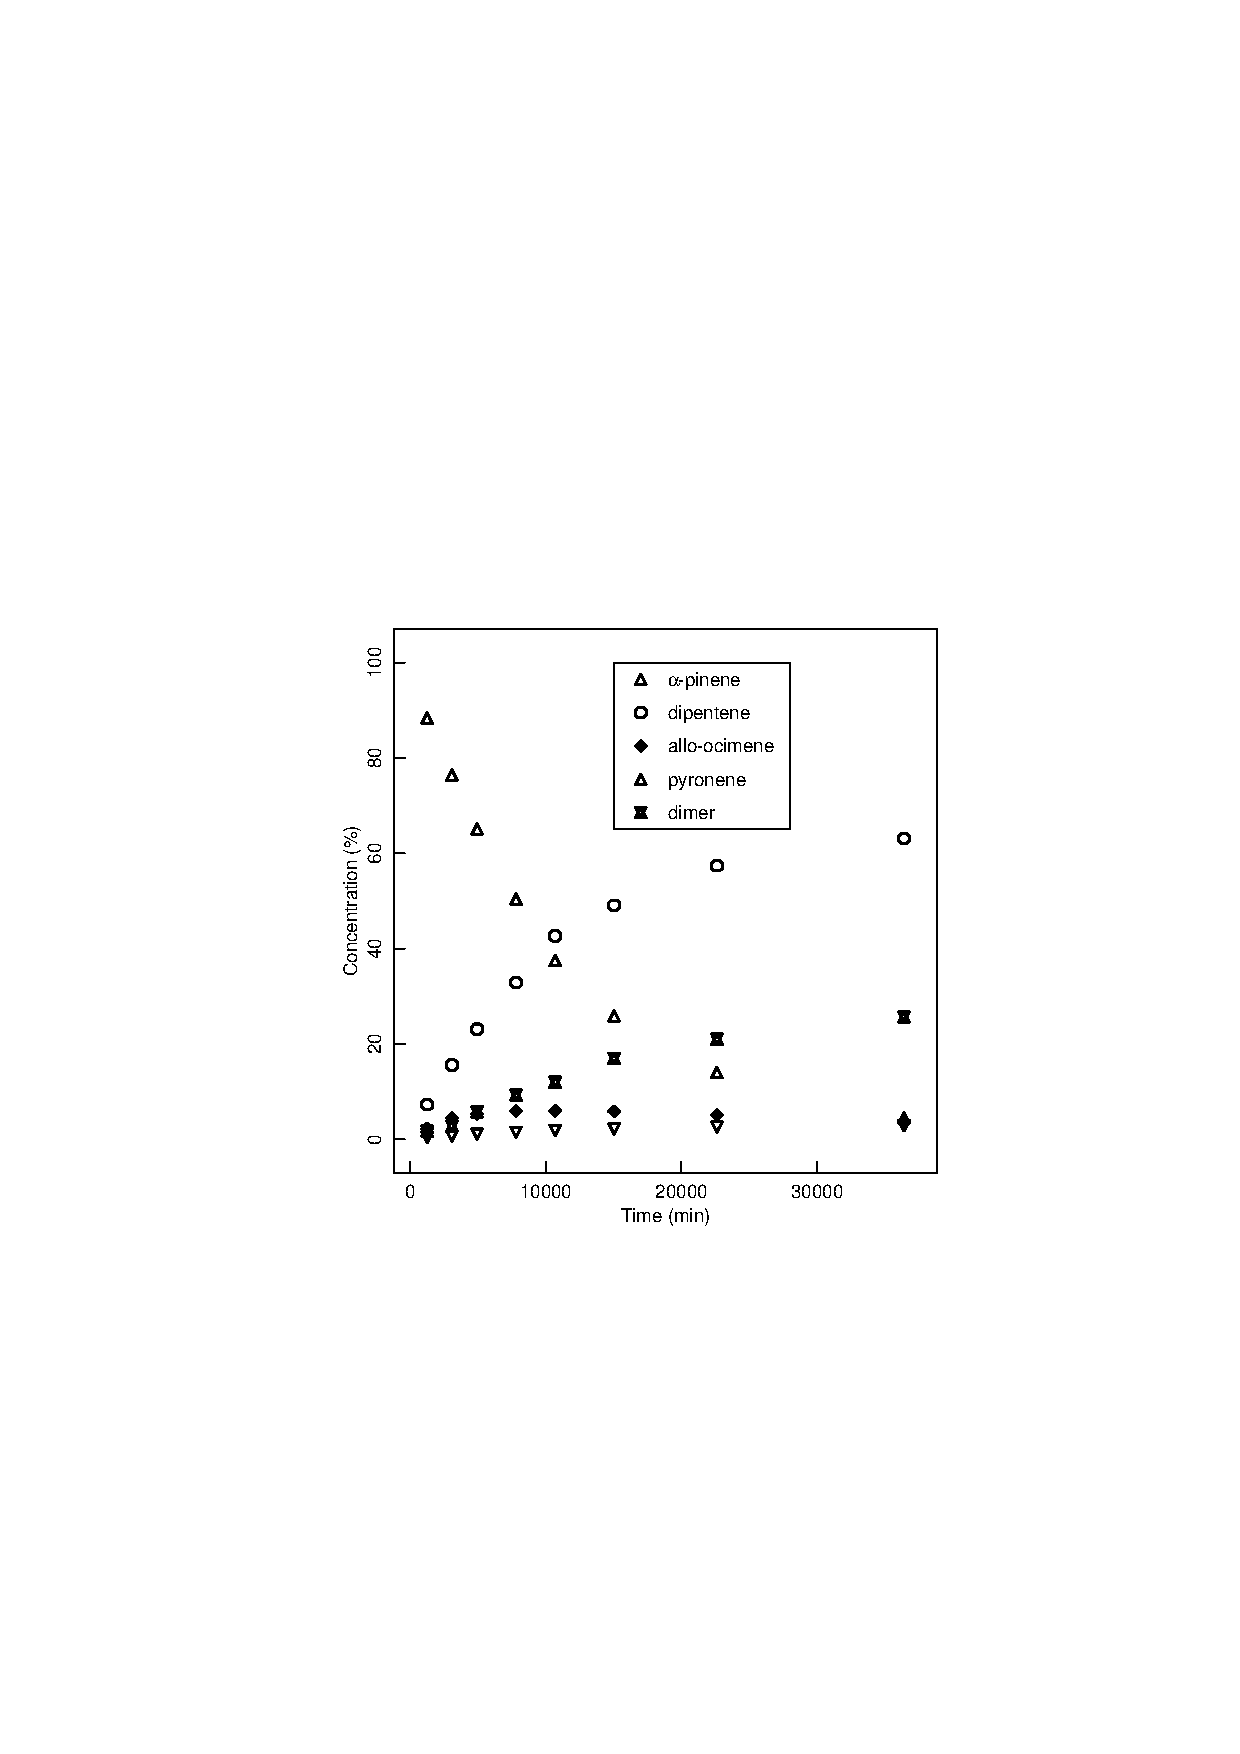
\includegraphics{4BHMEdata}}%,height=3in}}
    \caption{\label{fig:BHMEdata}
    Plot of the concentrations of
    $\alpha$-pinene and its by-products versus time at 189.5$^\circ$C.
    }
  \end{figure}
\end{example}

\begin{example}\label{spmma:1}
The behavior of the complex dielectric coefficient of a polymer
can be used to help understand the molecular structure of the
polymer.
Physically, a disk of the polymer is inserted between the two
metal electrodes of the dielectric cell which forms one arm of a
four armed electrical bridge.
The bridge is powered by an oscillating voltage whose frequency
($f$, in hertz) can be changed over a wide range (say 5 to 500000
Hz), and bridge balance is achieved using capacitance and
conductance standards.
The complex dielectric constant is then calculated using changes
from the standards relative to the cell dielectric constant.
Measurements are made by simultaneously adjusting the capacitance
(real) and the conductance (imaginary) arms of the bridge
when it is excited at a specific frequency and temperature.

The complex dielectric constant is written
$\epsilon * = \epsilon ' - i \epsilon ''$, where
$\epsilon '$ is the real component, $\epsilon ''$ is the
imaginary component, and $i$ denotes $\sqrt -1$.
\citeasnoun{havr:nega:1967}
%\glossary{ Havriliak, S. Jr.}
%\glossary{ Negami, S.}
analyzed the dielectric relaxation data for 21 polymers, and
proposed a general model of the form
  \begin{equation}\label{eqn:4.1}
    \epsilon *  =  \epsilon_{\infty} +
    {\epsilon_0-\epsilon_{\infty}\over\left[1+(i 2\pi f/f_0)^\alpha
    \right]^{\beta}}
  \end{equation}

In Figure~\ref{fig:PMMAdata}$a$ and $b$ we plot the imaginary component
  \begin{figure}
    \centerline{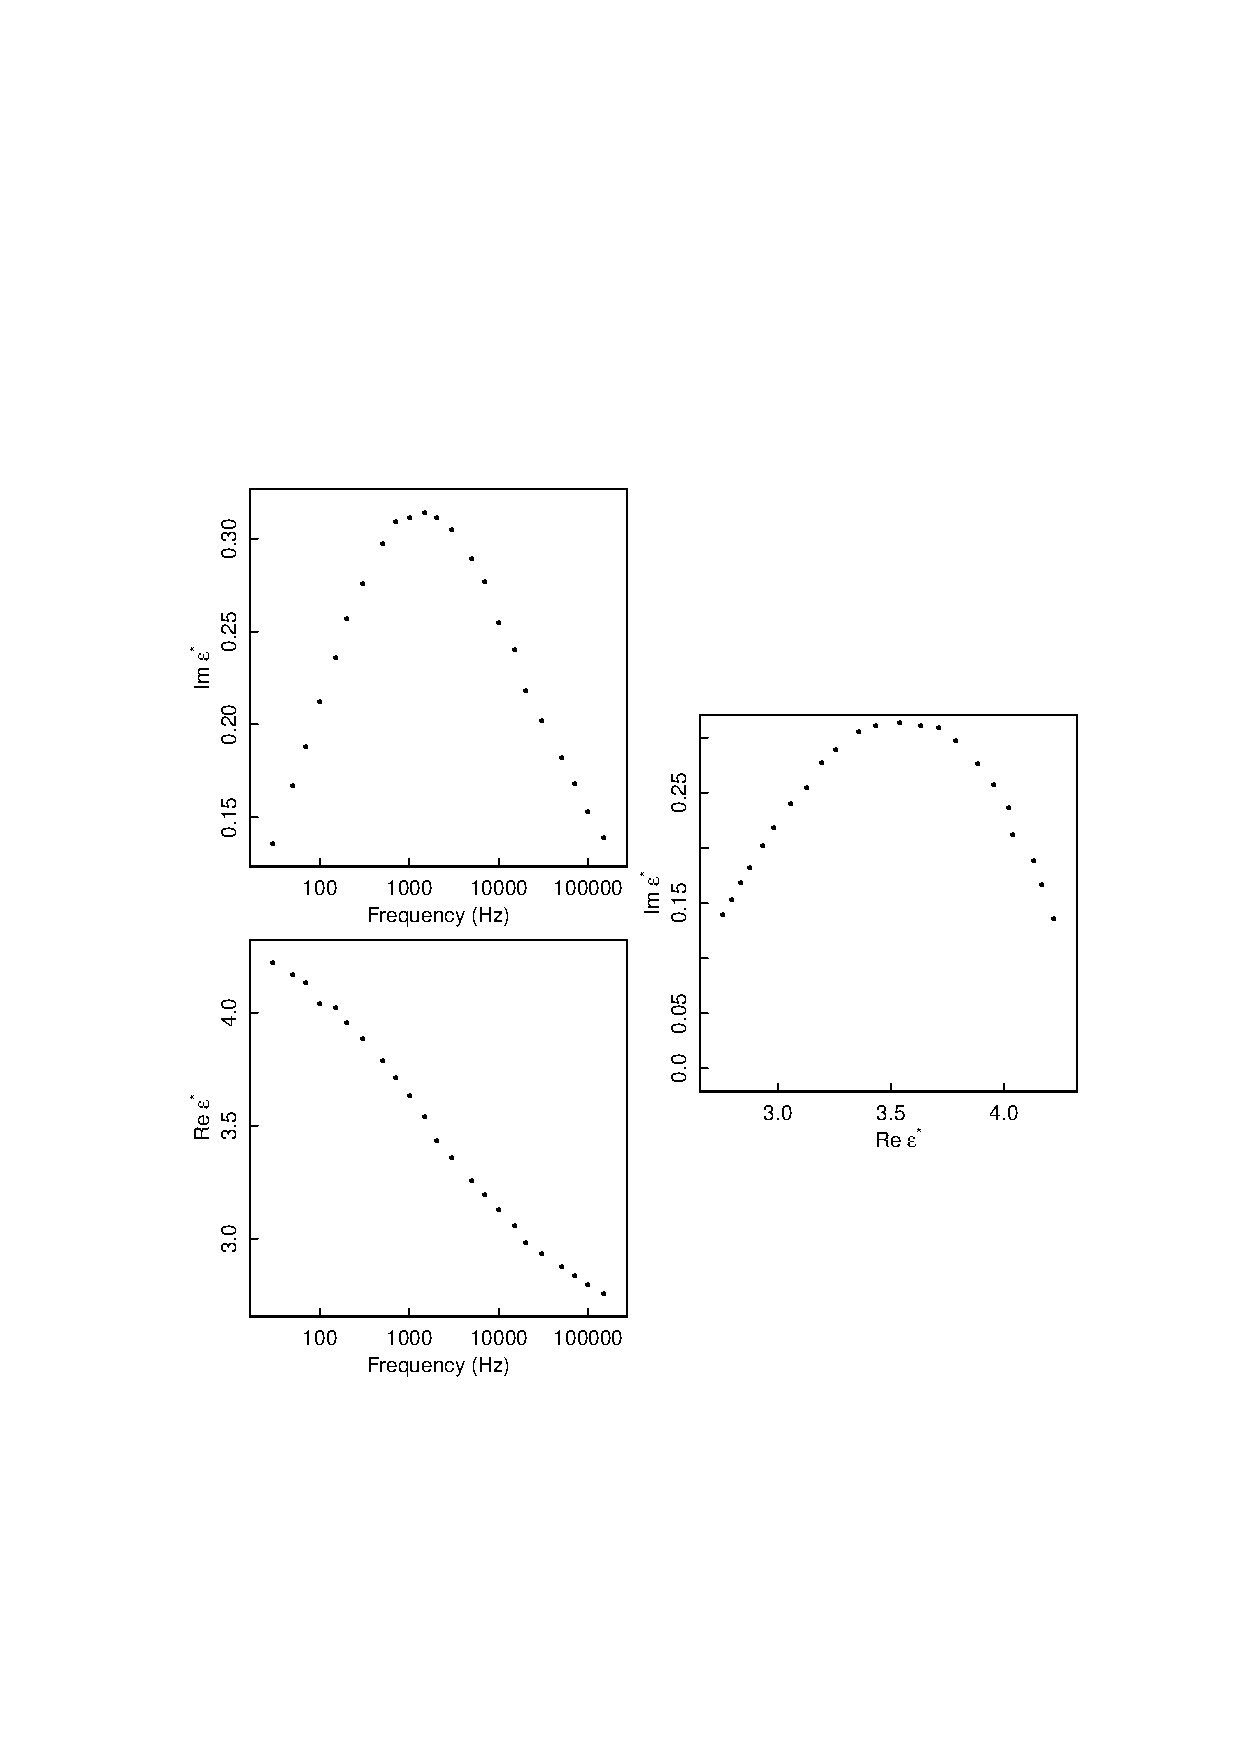
\includegraphics{4PMMAdata}}%,height=4in}}
    \caption{\label{fig:PMMAdata}
    Plots of the real and imaginary components of the dielectric constant
    $\epsilon^{*}$ (dimensionless)
    versus frequency (on a logarithmic scale) and in the complex
    plane for the s-PMMA dielectric data.
    }
  \end{figure}
$y_{\mbox{\it imag}}$ and the real component
$y_{\mbox{\it real}}$, versus frequency for syndiotactic
poly(methylmethacrylate) (s-PMMA) at 86.7$^\circ$F,
and, as recommended in \citeasnoun{cole:cole:1941},
%\glossary{ Cole, K.S.}
%\glossary{ Cole, R.H.}
in Figure~\ref{fig:PMMAdata}$c$ we plot these components in the complex
plane.
In this example, there are $M = 2$ responses, $N = 23$ cases,
and $P = 5$ parameters.
The data are listed in Appendix A, Section~\ref{atbl:spmma}.
\end{example}

As with uniresponse parameter estimation discussed in the
previous chapters, in the analysis of experimental data we assume
that the $N$ experimental design variables $ \bx_n $,
$n = 1 ,\ldots, N$, are fixed and known, so we can form the
$N \times M$ observation matrix $\bY$ with $(n,m)$th element
\index{matrix!observation}
$y_{nm}$ and the $N \times M$ expected response matrix
\index{matrix!expected response}
$\bH ( \btheta )$ with $(n,m)$th element
$ f_m ( \bx_n , \btheta )$.
From $\bY$ and $\bH ( \btheta )$, we create the residual matrix
\index{residual!matrix}
\index{matrix!residual}
\begin{equation}\label{eqn:4.3}
  \bZ ( \btheta ) = \bY - \bH ( \btheta )
\end{equation}

The parameter estimates $\hat{\btheta}$ are given by the values of
$\btheta$ which optimize some criterion based on
$\bZ ( \btheta )$ in the same
way that the least squares estimates in uniresponse parameter
estimation minimize $\norm \bz ( \btheta ) \norm^{2}$.
The criterion will depend on assumptions about the disturbance.
\index{assumptions!disturbance}
\index{assumptions!multiresponse}
For example, if we make the stringent assumption that the
${\rm Z}_{nm}$ are normally distributed and
independent with the same variance $\sigma^{2}$, then least squares
is appropriate and we find $\hat{\btheta}$ which minimizes
the sum of squared residuals of all $NM$ responses.
That is, the estimation criterion would be to minimize
the {\em trace\/}
of $\bZ \trans \bZ$, ${\rm \tr} ( \bZ \trans \bZ )$.
\index{trace!criterion for multiresponse estimation}

The assumptions leading to the trace criterion may not be
realistic.
It could be reasonable to assume that the variances of different
measurements on the same response are constant, but not that the
variances of different responses are equal.
Furthermore, assuming independent disturbances for different
measurements in the same experimental run may not be justified.
For example, in chemical experiments where the concentrations of
a number of different chemical species are measured from the same
sample, if only the relative concentrations can be determined,
different measurements on the same sample may be correlated.
Similarly, for dielectric determinations, errors in the frequency
settings can induce errors in both components.

Following \citeasnoun{box:drap:1965}, the model used to describe the
%\glossary{ Box, G.E.P.}
%\glossary{ Draper, N.R.}
disturbance term is a normal distribution with
$$
\mbox{\rm E} [ {\rm Z}_{nm} ] = 0
$$
and
$$
\mbox{\rm E} [ {\rm Z}_{nm} {\rm Z}_{ri} ] = \left\{
\begin{array}{c l}
  \{\bSIGMA\}_{mi}&n=r\\
  0&n\ne r
\end{array}\right.
$$
where $\bSIGMA$ is a fixed $M \times M$ covariance matrix.
\index{covariance!matrix}
\index{matrix!covariance}
That is, we
assume that measurements from different experiments are
independent but measurements from the same experiment are correlated.
The joint probability density function
for the $N$ observations, conditional on
all the unknown parameters, is then
\begin{eqnarray}\label{eqn:4.4}
  p(\bY|\btheta,\bSIGMA)&\sim&
  | \bSIGMA |^{- N/2}
  \exp\left[-{\tr[(\bY-\bH)\bSIGMA^{-1}(\bY-\bH)\trans]\over 2}\right]\\
  &=& | \bSIGMA^{-1} |^{N/2} \exp
  \left[ -{\tr ( \bZ \bSIGMA^{-1} \bZ \trans ) \over 2 }\right]\nonumber
\end{eqnarray}
where the vertical bars denote a determinant.

\subsection{The Determinant Criterion}
\index{determinant!criterion for multiresponse estimation}

A parameter estimation criterion under these assumptions can be
derived using a likelihood or Bayesian argument.
The loglikelihood function for the parameters $\btheta$ and
$\bSIGMA^{-1}$ is
\begin{equation}\label{eqn:4.5}
  L ( \btheta ,  \bSIGMA^{-1} ) = k + {N \over 2 }\ln | \bSIGMA^{-1} |-
  {\tr ( \bZ\bSIGMA^{-1} \bZ \trans ) \over 2 }
\end{equation}
where $k$ is an unimportant constant.
To maximize the loglikelihood function we write the last term as
${\rm \tr} ( \bZ \trans \bZ \bSIGMA^{-1} )$ and
differentiate the entire expression with
respect to the elements $\sigma^{mi}$ of $\bSIGMA^{-1}$.
Using the result \cite[p.~296]{bard:1974}
%\glossary{ Bard, Y.}
\begin{equation}\label{eqn:4.6}
  {\partial \ln | \bSIGMA^{-1} | \over \partial \sigma^{mi}}=
  \lb \bSIGMA \rb_{mi}
\end{equation}
allows us to write
$$
{\partial L ( \btheta , \bSIGMA^{-1} ) \over \partial \sigma^{mi}}=
{N \over 2 }\{\bSIGMA\}_{mi}{-1\over 2}\{\bZ\trans\bZ\}_{mi}
$$
Setting this derivative to zero provides the conditional estimates
$$
\lb \hat{\bSIGMA}( \btheta ) \rb_{mi}={\lb \bZ \trans \bZ \rb_{mi} \over N }$$
or
$$
\hat{\bSIGMA}( \btheta )={\bZ \trans \bZ \over N }$$
which, when substituted into (\ref{eqn:4.5}), gives the conditional loglikelihood
\index{loglikelihood!conditional}
function
\begin{equation}\label{eqn:4.7}
  L ( \btheta ,  \hat{\bSIGMA}( \btheta ) ) =
  k' - {N \over 2 }\ln | \bZ \trans \bZ |
\end{equation}
The maximum likelihood estimates are then obtained
\index{maximum likelihood estimate}
by minimizing $| \bZ \trans \bZ |$ with respect to $\btheta$.

A Bayesian argument was used by
\citeasnoun{box:drap:1965} to derive
%\glossary{ Box, G.E.P.}
%\glossary{ Draper, N.R.}
the marginal posterior density for $\btheta$ by integrating over
the unknown variances and covariances after incorporating an
noninformative prior of the form
$$
p ( \bSIGMA ,  \btheta ) \sim
| \bSIGMA |^{ - ( M + 1 ) /2 }
$$
The marginal posterior density is then
\begin{equation}\label{eqn:4.8}
  p ( \btheta | \bY ) \sim | \bZ \trans \bZ |^{{-} N/2}
\end{equation}
and so the posterior density is maximized when the determinant is
minimized.
Thus, the likelihood and Bayesian approaches lead to the same
criterion.

As pointed out in \citeasnoun{box:tiao:1973},
%\glossary{ Box, G.E.P.}
%\glossary{ Tiao, G.C.}
(\ref{eqn:4.7}) and (\ref{eqn:4.8}) are
remarkably general results, since they do not depend on whether
the expectation functions are linear or nonlinear, whether the
parameters are common to more than one response, or whether the
design variables are common to more than one response.
Furthermore, a scale change on any of the responses will not
affect the estimates, and linear combinations of the responses
can be used in place of the original responses.

Geometrically, $| \bZ \trans \bZ |$ corresponds to the square of the
\index{geometry!of multiresponse determinant criterion}
volume of the $M$-dimensional parallelepiped spanned by the residual
vectors,
\index{residual!vector}
$\bz_m ,m=1 ,\ldots, M$,
in the $N$-dimensional case space.
Minimizing the determinant corresponds to minimizing the volume
enclosed by the residual vectors.

\subsection{Inferences for Multiresponse Estimation}
\index{inference!in multiresponse estimation}

To draw inferences about parameters in multiresponse estimation,
we use the Bayesian formulation and
assume that $| \bZ \trans \bZ |$ can be
adequately represented by a quadratic Taylor series near
$\hat{\btheta}$ to give an approximate marginal posterior density function.
From (\ref{eqn:4.8}),
\begin{equation}\label{eqn:4.9}
  p(\btheta|\bY)\approx\left[{1+(\btheta-\hat{\btheta})\trans
  { { \bOMEGA   \over  2 | \hat{\bZ}\trans \hat{\bZ}| } }
  ( \btheta - \hat{\btheta}) }\right]^{{-}N/2}
\end{equation}
where $\bOMEGA$ is the Hessian of the determinant evaluated at
\index{Hessian!of determinant}
$\hat{\btheta}$.
This approximation has the form of a
$P$-variate Student's T density with location parameter
\index{T distribution!multivariate}
$\hat \btheta$, degrees of freedom $N-P$, scale factor
\begin{equation}\label{eqn:4.101}
  s^2 = {| \hat{\bZ}\trans \hat{\bZ}|} / (N - P)
\end{equation}
and covariance matrix
$2 s^2 \bOMEGA^{-1}$ \cite{box:tiao:1973}.
%\glossary{ Box, G.E.P.}
%\glossary{ Tiao, G.C.}
An approximate $1 - \alpha $ HPD region for
\index{highest posterior density (HPD)!approximate region in multiresponse estimation}
the parameters is given by
\begin{equation}\label{eqn:4.10}
  ( \btheta - \hat \btheta ) \trans
  {\bOMEGA  \over 2 }( \btheta - \hat \btheta )  \le 
  P s^2 \FPNP
\end{equation}
so that the square of the volume in the parameter space enclosed by
the joint region is proportional to the determinant of the Hessian.

Because we are approximating $| \bZ \trans \bZ |$, the
approximations (\ref{eqn:4.9}) and (\ref{eqn:4.10}) may be very poor:
additional research needs to be done to assess the adequacy of
these approximations even for cases where the model functions
are linear.
More accurate HPD regions can be written as either
\begin{equation}\label{eqn:Fregion}
  {( | \bZ \trans \bZ |-| \hat \bZ \trans \hat \bZ | ) / P \over s^2 }\FPNP
\end{equation}
or
\begin{equation}\label{eqn:Chiregion}
  \ln [p ( \hat \btheta | \bY ) ] - \ln [p ( \btheta | \bY ) ] 
  {1 \over 2 }\chi^2 ( P ; \alpha )
\end{equation}
\cite{box:tiao:1973}, where $\chi^2 ( P ; \alpha )$ is the upper
%\glossary{ Box, G.E.P.}
%\glossary{ Tiao, G.C.}
$\alpha$ percentile of the $\chi^{2}$ distribution with $P$
degrees of freedom.
Such regions would have to be determined numerically and
displayed in contour plots, and therefore suffer from the
disadvantages inherent in exact confidence and likelihood
regions for uniresponse models, as discussed in Chapter 6.
Nevertheless, the methods of Chapter 6 (profile $t$ and profile trace
plots) can be used for multiresponse problems.

An approximate $1 - \alpha $ HPD interval for the
\index{highest posterior density (HPD)!approximate interval in multiresponse estimation}
parameter $\theta_{p}$ is given by
\begin{equation}\label{eqn:4.12}
  \hat \theta_p\pm\tNP s \sqrt{2 \lb \bOMEGA^{-1} \rb_{pp}}
\end{equation}
and an approximate $1 - \alpha $ HPD band for the
\index{highest posterior density (HPD)!approximate band in multiresponse estimation}
$m$th expectation function $f_m ( \bx , \btheta )$ is
$$
f_m(\bx,\hat \btheta )\pm s\sqrt{2\bv_m \trans\bOMEGA^{-1} \bv_m}
\sqrt{P\FPNP}
$$
where $\bv_{m}$ is the gradient of $f_{m}$
with respect to $\btheta$ evaluated at $\bx$ and $\hat{\btheta}$.

\subsection{Dimensional Considerations in Multiresponse Estimation}

Note that the determinant criterion implies two important
constraints on the
\index{determinant!constraints for multiresponse estimation}
\index{constraint!in multiresponse estimation}
number of observations, $N$, the number of responses, $M$, and
the number of parameters, $P$.

First, $M$ can not exceed $N$, since otherwise the determinant is
identically zero.
To see this, note that the rank of the $N \times M$ matrix $\bZ$
cannot exceed the minimum of $( N , M )$, and when $NM$ the
rank of the $M \times M$ matrix $\bZ \trans \bZ$ is less than $M$ and
hence the determinant is identically zero.
Another way of seeing this is to recall from the geometric interpretation
that $| \bZ \trans \bZ |$
gives the square of the volume, in the $N$-dimensional case space,
enclosed by the residual vectors (columns of $\bZ$).
If the case dimension $N$ does not at least equal the
response dimension $M$, then the volume is zero.
For example, the volume of a rectangle is zero.

Second, in general $P$ must be less than $N$,
since otherwise the criterion
can be made zero by fitting any one response perfectly, or even by
fitting a linear combination of the responses perfectly.
That is, if there is an $M$-vector $\bv$ such that
$\bZ(\btheta)\bv=\boldsymbol{0}$ for some $\btheta$, then the determinant will
be zero at that value of $\btheta$ regardless of how well the
remaining responses have been fitted.

The reasoning leading to the constraint $N>P$ provides
justification for the use of $N-P$ for the residual degrees of
freedom proposed above.
It would seem that with $NM$ data values there
should be $N M - P$ degrees
of freedom for the residuals, as suggested in
\citeasnoun{bard:1974}, but in fact, near the
%\glossary{ Bard, Y.}
optimum the value of the determinant is controlled by the linear
combination of responses corresponding to the smallest singular
value of $\bZ$, and this vector has dimension $N$.
The vector corresponding to this singular value
therefore has $N - P$ degrees of freedom.

In summary, the number of cases, $N$, should exceed the maximum of $M$
and $P$ to ensure a successful analysis.

A great advantage in using multiresponse data is the increased
\index{multiresponse estimation!advantages and disadvantages}
precision of parameter estimates relative to those obtained from
uniresponse data.
However, we cannot attribute this increased precision to additional
denominator degrees of freedom when multiple responses are used.
The increased precision is due to the combination of different
types of information from the responses.

One difficulty with the use of multiresponse data is that
all problems become nonlinear optimization problems.
That is, even if the expectation functions are linear in the parameters,
iterative methods must be used to obtain the estimates which minimize
the determinant criterion.
The problem of obtaining the best estimates is also more difficult
than in the uniresponse nonlinear case, since the Hessian need not
be positive definite.
Further discussion on these aspects of optimizing the determinant
is given in Section 4.2.3.

Another difficulty with multiresponse estimation is that
inference regions for the parameters based on (\ref{eqn:4.10})
or (\ref{eqn:4.12}) are only approximate, even when all the
expectation functions are linear in the parameters.
The accuracy of these approximations is questionable.
On the other hand, inference regions from multiresponse
estimation are usually much smaller than those from uniresponse
estimation, and so approximate multiresponse regions may in fact
be better than approximate uniresponse regions for nonlinear models.

In spite of the difficulties,
multiresponse estimation is a valuable
technique and should be used whenever multiresponse data are available.
The reduction in size of the parameter inference regions,
together with the extra ability to discriminate between rival models,
is well worth any additional effort required.

\section{A Generalized Gauss--Newton Method}

One advantage of least squares as a criterion is that
specialized methods can be used to exploit properties of the
criterion and to provide standard optimization algorithms.
In this section, we describe a Gauss--Newton method for minimizing the
determinant criterion.

To evaluate the determinant, following \citeasnoun{bate:watt:1987},
%\glossary{ Bates, D.M.}
%\glossary{ Watts, D.G.}
\index{determinant!evaluation by QR decomposition}
we take a {\it QR} decomposition of $\bZ ( \btheta )$,
\index{QR decomposition!of residual matrix}
$$
\bZ ( \btheta ) = \bQ \bR = \bQ_1 \bR_1
$$
Then, since
\begin{eqnarray*}
  | \bZ ( \btheta ) \trans  \bZ ( \btheta ) |&=&| \bR_1 \trans \bR_1 |\\
  &=&| \bR_1 |^2\\
  &=&\prod_{m=1}^M\{\bR_1\}_{mm}^2
\end{eqnarray*}
we have  an  easy  way  to  evaluate  the  determinant
criterion for any  $\btheta$.

\subsection{The Gradient and Hessian of the Determinant}

The decomposition of $\bZ ( \btheta )$ as $\bQ_1 \bR_1 $ is
also helpful in evaluating the gradient and Hessian of the
determinant criterion.
To simplify notation we omit the dependence on
$\btheta$ and use a subscript enclosed in parentheses to
denote differentiation, as
$$
{ \partial \bZ   \over  \partial \theta_p } = \bZ_{(p)}
$$
Using the result (1.1.34) from \citeasnoun{fedo:1972},
%\glossary{ Fedorov, V.V.}
we have
\begin{equation}\label{eqn:4.14}
  {\partial | \bZ \trans \bZ |  \over \partial \theta_p } =
  | \bZ \trans \bZ |  \tr \left[ ( \bZ \trans \bZ )^{-1}
  {\partial ( \bZ \trans \bZ )  \over \partial \theta_p }
  \right]
\end{equation}
with
\begin{equation}\label{eqn:4.15}
  { \partial ( \bZ \trans \bZ )   \over  \partial \theta_p } =
  \bZ \trans \bZ_{(p)} + \bZ_{(p)} \trans \bZ
\end{equation}
so the gradient
\index{gradient!of determinant}
\index{determinant!gradient of}
$\bomega = \partial | \bZ \trans \bZ | / \partial \btheta \trans$
has components
\begin{eqnarray}\label{eqn:4.16}
  \lb \bomega \rb_p
  &=&2 | \bZ \trans \bZ |   \tr [ ( \bZ \trans \bZ )^{-1} \bZ \trans \bZ_{(p)} ]\\
  &=& 2 | \bZ \trans \bZ | \tr [ \bR_1^{-1} \bR_1 \invtrans
  \bR_1 \trans \bQ_1 \trans \bZ_{(p)} ]\nonumber\\
  &=& 2 | \bZ \trans \bZ |  \tr [ \bR_1^{-1} \bQ_1 \trans \bZ_{(p)} ]\nonumber\\
  &=& 2 | \bZ \trans \bZ |  \tr [ \bZ^+ \bZ_{(p)} ]\nonumber
\end{eqnarray}
where $\bZ^+ = \bR_1^{-1} \bQ_1 \trans$ is the
pseudoinverse of $\bZ$.

To obtain the second derivative or Hessian terms, we write
\index{Hessian!of determinant}
\index{determinant!Hessian of}
\begin{equation}\label{eqn:4.17}
  g = \ln | \bZ \trans \bZ |
\end{equation}
so that
\begin{equation}\label{eqn:4.17a}
  | \bZ \trans \bZ | = e^g
\end{equation}
and
\begin{equation}\label{eqn:4.18}
  g_{(p)} = 2  \tr [ \bZ^+ \bZ_{(p)} ]
\end{equation}
and then use the expressions for the derivative of the pseudoinverse
\cite{golu:pere:1973} to obtain
%\glossary{ Golub, G.H.}
%\glossary{ Pereyra, V.}
\begin{eqnarray}\label{eqn:4.19}
  g_{(pq)}&=&
  2 \lb - \tr [ \bZ^+ \bZ_{(p)} \bZ^+ \bZ_{(q)} ] +
  \tr [ \bZ^+ ( \bZ^+ ) \trans \bZ_{(p)} \trans
  ( \bI - \bZ \bZ^+ ) \bZ_{(q)} ]\\
  &&+\tr [ \bZ^+ \bZ_{(pq)} ] \rb\nonumber
\end{eqnarray}
From (\ref{eqn:4.17a}), a second derivative term for
$| \bZ \trans \bZ |$ is then
\begin{equation}\label{eqn:omega}
  {\partial^2 | \bZ \trans \bZ |  \over \partial \theta_p \partial \theta_q} =
  | \bZ \trans \bZ | [ g_{(p)} g_{(q)} + g_{(pq)} ]
\end{equation}

Alternative expressions for the gradient and Hessian of
$| \bZ \trans \bZ |$ are obtained by expanding (\ref{eqn:4.16}) as
\begin{eqnarray}\label{eqn:4.21}
  \lb \bomega \rb_p&=&
  | \bZ \trans \bZ | \tr [ ( \bZ \trans \bZ )^{-1}
  ( \bZ \trans \bZ_{(p)}+\bZ_{(p)} \trans \bZ ) ]\\
  &=&| \bZ \trans \bZ | \tr [ \bU_p ]\nonumber
\end{eqnarray}
where
$\bU_p = ( \bZ \trans \bZ )^{-1}
( \bZ \trans \bZ_{(p)} + \bZ_{(p)} \trans \bZ ) $.
Differentiating (\ref{eqn:4.21}) with respect to $\theta_{q}$ gives
\begin{eqnarray}\label{eqn:4.22}
  {\partial^2 | \bZ \trans \bZ | \over \partial \theta_q \partial \theta_p }&=&
  \lb \bomega \rb_q \tr [ \bU_p ]+| \bZ \trans \bZ | \lb
  - \tr [ \bU_q \bU_p ] +
  \tr [ ( \bZ \trans \bZ )^{-1}
  ( \bZ_{(q)} \trans \bZ_{(p)} + \bZ_{(p)} \trans \bZ_{(q)} ) ]\\
  &&+\tr [ ( \bZ \trans \bZ )^{-1}
  ( \bZ \trans \bZ_{(pq)}+\bZ_{(pq)} \trans \bZ ) ] \rb\nonumber\\
  &=&| \bZ \trans \bZ | \lb \tr [ \bU_q ] \tr [ \bU_p ]-
  \tr [ \bU_q \bU_p ]+
  \tr [ ( \bZ \trans \bZ )^{-1}
  ( \bZ_{(q)} \trans \bZ_{(p)}+\bZ_{(p)} \trans \bZ_{(q)} ) ]\nonumber\\
  &&+
  \tr [ ( \bZ \trans \bZ )^{-1}
  ( \bZ \trans \bZ_{(pq)}+\bZ_{(pq)} \trans \bZ ) ] \rb\nonumber\\
\end{eqnarray}

\subsection{An Approximate Hessian}
\index{Hessian!approximate}

The last term in the expression for $g_{(pq)}$
requires second derivatives of the model functions.
We prefer to avoid calculating second derivatives, especially
since the Hessian matrix is being used primarily to determine an
increment, and so we make the same assumption as in the
Gauss--Newton method for nonlinear least squares.
That is, we assume that the model functions can be locally
approximated by linear functions and set
$\bZ_{(pq)} $ to zero.
The {\em approximate Hessian\/} matrix $\bOMEGA$ is therefore
calculated with entries
\begin{eqnarray}\label{eqn:4.20a}
  \lb \bOMEGA \rb_{pq}&=&4 | \bZ \trans \bZ |
  \tr [ \bZ^+ \bZ_{(p)} ]\tr [ \bZ^+ \bZ_{(q)} ]\\
  &&+2 | \bZ \trans \bZ | \lb - \tr [ \bZ^+ \bZ_{(p)}
  \bZ^+ \bZ_{(q)} ]
  +\tr [ \bZ^+ ( \bZ^+ ) \trans \bZ_{(p)} \trans
  ( \bI-\bZ \bZ^+ ) \bZ_{(q)} ] \rb\nonumber\\
\end{eqnarray}
These can be collected into $\bOMEGA$ and used with the gradient vector
$\bomega$ to form the increment $\bdelta=- \bOMEGA^{-1} \bomega$ in a
Newton--Raphson iterative scheme to optimize $| \bZ \trans \bZ |$.
Since only first derivatives of the model functions
are used, this is a generalization
of the Gauss--Newton method for nonlinear least squares.
\index{Gauss--Newton!method for multiresponse estimation}

Some rearrangement of the terms in (\ref{eqn:4.16}) and
(\ref{eqn:4.19}) can be used
to simplify the calculations of $\bomega$ and $\bOMEGA$
\cite{bate:watt:1984}.
%\glossary{ Bates, D.M.}
%\glossary{ Watts, D.G.}
In particular, we can use the relationship
$\tr ( \bA \bB ) = \tr ( \bB \bA )$ to change (\ref{eqn:4.16}) to
\begin{eqnarray}\label{eqn:4.24}
  \lb \bomega \rb_p&=&
  2 | \bZ \trans \bZ |\tr [ \bQ_1 \trans \bZ_{(p)} \bR_1^{-1} ]\\
 &=&2 | \bZ \trans \bZ | \sum_{m=1}^M { g_{p,mm} }\nonumber
\end{eqnarray}
where $g_{p,mm}$ is the $(m,m)$th element of the
$N \times M$ matrix
\begin{equation}\label{eqn:4.24a}
  \bG_p = \bQ \trans \bZ_{(p)} \bR_1^{-1}
\end{equation}
This does not change the gradient calculation substantially, but
now (\ref{eqn:4.20a}) can be rewritten to give
\begin{eqnarray}\label{eqn:4.25}
  \lb \bOMEGA \rb_{pq}&=&4 | \bZ \trans \bZ | \sum_{m=1}^M
  { g_{p,mm} } \sum_{m=1}^M { g_{q,mm} }\\
  &&+2 | \bZ \trans \bZ | \lb - \tr [ \bQ_1 \trans \bZ_{(p)}
  \bR_1^{-1}  \bQ_1 \trans \bZ_{(q)} \bR_1^{-1} ]\nonumber\\
  &&+\tr [ \bR_1^{-1} \bQ_1 \trans \bQ_1
  \bR_1^{{{\rm }} -T}\bZ_{(p)} \trans \bQ_2 \bQ_2 \trans \bZ_{(q)} ]
  \rb\nonumber\\
  & = & 4 | \bZ \trans \bZ | \sum_{m=1}^M
  {g_{p,mm}}\sum_{m=1}^{M{g}_{q,mm}}\nonumber\\
  &&+ 2 | \bZ \trans \bZ | \left( - \sum_{m=1}^M
  \sum_{i=1}^M g_{p,mi} g_{q,im} +
  \tr [ ( \bQ_2 \trans \bZ_{(p)} \bR_1^{-1} ) \trans
  ( \bQ_2 \trans \bZ_{(q)} \bR_1^{-1} ) ] \right)\nonumber\\
  &=&4 | \bZ \trans \bZ | \sum_{m=1}^M
  g_{p,mm} \sum_{m=1}^M g_{q,mm}\nonumber\\
  &&+ 2 | \bZ \trans \bZ | \left( - \sum_{m=1}^M
  \sum_{i=1}^M {g_{p,mi} g_{q,im}} +
  \sum_{m=M+1}^N 
  \sum_{i=1}^M {g_{p,mi} g_{q,mi}} \right)
\end{eqnarray}
Equation (\ref{eqn:4.25}) permits very efficient evaluation of $\bOMEGA$,
because once the $QR$ decomposition of $\bZ$ is done and
the matrices $\bG_p ,  p = 1 ,\ldots, P$, are formed, it is only
necessary to collect a few inner products.
As discussed in Appendix 2, although $\bQ \trans$ occurs as a factor
in (\ref{eqn:4.24a}),
the matrix $\bQ$ is not explicitly formed; instead, a product
such as $\bQ \trans \bZ_{(p)} $ is formed by applying
Householder transformations to $\bZ_{(p)} $.

\subsection{Calculations for Each Iteration}

At each iteration, the current value of the parameter vector,
$\btheta^{0}$, is used to evaluate $| \bZ \trans \bZ |$, the gradient
$\bomega$, and the approximate Hessian $\bOMEGA$.
If $\bOMEGA$ is positive definite, the increment is calculated by
\index{Gauss--Newton!increment for multiresponse estimation}
solving
\begin{equation}\label{eqn:4.23a}
  \bOMEGA \bdelta^0 = - \bomega
\end{equation}
for $\bdelta^{0}$ and setting
$$
\btheta^1 =  \btheta^0 + \lambda \bdelta^0
$$
where $\lambda$ is a step size factor chosen to ensure that
\index{step factor}
$ | \bZ ( \btheta^1 ) \trans \bZ ( \btheta^1 ) | 
| \bZ ( \btheta^0 ) \trans \bZ ( \btheta^0 ) |$.
The solution to (\ref{eqn:4.23a}) is accomplished most efficiently by taking
a Cholesky decomposition of $\bOMEGA$ \cite[Chapter 8]{dong:bunc:mole:stew:1979} as
%\glossary{ Dongerra, J.J.}
%\glossary{ Bunch, J.R.}
%\glossary{ Moler, C.B.}
%\glossary{Stewart, G.W.}
\index{Cholesky!decomposition}
\begin{equation}\label{eqn:cholesky}
  \bOMEGA = \bC \trans \bC
\end{equation}
where $\bC$ is $P\times P$ and upper triangular.

Unlike the Gauss--Newton method for nonlinear least squares, the
generalized Gauss--Newton method for multiresponse data need not
result in a positive definite $\bOMEGA$.
\index{Hessian}
One of the situations in which negative eigenvalues of the Hessian can
occur is when there are multiple minima for the determinant criterion,
such as in the case study of Section 5.5.

When $\bOMEGA$ is not positive definite, the quadratic
approximation to $| \bZ \trans \bZ |$ does
not have a minimum and $\bC$ cannot
be calculated.
As in Section 3.5, we restore positive definiteness to the
Hessian by inflating the diagonal and
modifying the increment to be the solution of
$$
( \bOMEGA + k \bI ) \bdelta^0 = - \bomega
$$
where $k$ is large enough to make $\bOMEGA + k \bI$ positive
definite.
Such a $k$ can be calculated by determining the eigenvalues of
$\bOMEGA$ and setting $k$ to twice the magnitude of the most
negative eigenvalue, or by using a modified Cholesky
decomposition \citeasnoun{denn:schn:1983}.
%\glossary{ Dennis, J.E.Jr.}
%\glossary{ Schnabel, R.B.}

\subsection{A Multiresponse Convergence Criterion}
\index{multiresponse estimation!convergence criterion}

To decide whether we have convergence at a particular parameter
vector $\btheta^{0}$, we reason as in Section 2.2.3 and compare the
magnitude of the increment at that point with the statistical
variability in the estimates.
The statistical variability is accounted for in the elliptical regions
of (\ref{eqn:4.10}), and so we take a linear transformation of the
parameters to make the regions spherical.
With such a transformation, the length of the increment
from $\btheta^{0}$ is simply $\norm \bC \bdelta \norm$, where $\bC$ is the
Cholesky factor from (\ref{eqn:cholesky}), and the region is
simply a disk with radius proportional to
$s\sqrt{P\FPNP}$.
The convergence criterion is then \cite{bate:watt:1987}
%\glossary{ Bates, D.M.}
%\glossary{ Watts, D.G.}
\index{convergence!criterion for multiresponse estimation}
$$
{ \norm \bC \bdelta \norm^2 / P   \over  2 s^2 }  \epsilon^2
$$
where $\epsilon$ is the tolerance level and $s^{2}$ is the scale
factor (\ref{eqn:4.101}).
When the criterion is small, it indicates that the requested
increment is negligible relative to the statistical variability.
The value of $\epsilon$ can be set at 0.001, reasoning as in
Section 2.2.3.

Pseudocode for multiresponse parameter estimation is presented in
Appendix 3, Section A3.3.

\section{Practical Considerations}
\index{practical considerations!in multiresponse estimation}
\index{multiresponse estimation!practical considerations}

As in uniresponse estimation, care should be taken in selecting the
model and obtaining starting estimates for the parameters.
After convergence, residuals for all the responses should be
examined using plots as described in Chapter 3.
However, multiresponse modeling involves additional practical
considerations, as discussed below.

\subsection{Obtaining Starting Values}
\index{starting values!multiresponse}

The techniques for obtaining starting estimates for uniresponse
models described in Chapter 3 can be used for multiresponse
models by applying the procedures to each response and
then combining the estimates to give starting values for the complete
parameter vector.
Graphical analyses can be especially helpful, as illustrated in
the following example.

\begin{example}\label{spmma:graph}
Starting estimates for the parameters in the expectation
function for the complex dielectric coefficient can be obtained
from graphical considerations, following \citeasnoun{havr:nega:1967}.
%\glossary{ Havriliak, S.Jr.}
%\glossary{ Negami, S.}
They showed that the real and imaginary components can be written
  \begin{eqnarray*}
    \epsilon'&=&\epsilon_{\infty} +
    ( \epsilon_0 - \epsilon_{\infty} ) R^{ - \beta }  \cos\beta \phi\\
    \epsilon''&=&
( \epsilon_0 - \epsilon_{\infty} ) R^{{-} \beta}  \sin\beta \phi
  \end{eqnarray*}
where
$$
R^2 =
\left[ 1 + ( 2 \pi f / f_0 )^{\alpha}
\cos ( \pi \alpha / 2 )\right]^2
+ \left[ ( 2 \pi f / f_0 )^{\alpha}
\sin ( \pi \alpha / 2 )\right]^2
$$
and
$$
\phi = \arctan \left[
{ ( 2 \pi f / f_0 )^{\alpha}
\sin ( \pi \alpha / 2 )  
\over   1+( 2 \pi f / f_0 )^{\alpha}
\cos ( \pi \alpha / 2 ) }\right]
$$
The parameters $\epsilon_{0}$ and $\epsilon_{\infty}$ are the
limiting low and high frequency intercepts of the locus with the
real axis, when the function is plotted in the complex plane.
Furthermore, the limiting angle the high frequency locus makes
with the real axis is
$ \psi_L = \pi \alpha \beta / 2 $, and the angle
bisector of $ \psi_L $ from $( \epsilon_{\infty} , 0 )$ intersects the
locus at the frequency $\tilde f $ for which
$2 \pi \tilde f / f_0 = 1$.
And finally, $\alpha$ is related to $ \psi_L $
through
$$
\psi_L = - \pi \alpha
{ \ln \left( \tilde {R \over  \epsilon_0 - \epsilon_{\infty} }\right)  
\over \ln[ 2+2\cos( \pi \alpha / 2 ) ]}
$$
where $\tilde R $ is the length of the line from
$( \epsilon_{\infty} , 0 )$ to $\epsilon * ( \tilde f ) $.

To obtain starting values for the s-PMMA data, we plotted the data
in the complex plane, as in Figure \ref{fig:PMMAdata}$c$, but this time we
made the scales of the real and imaginary parts equal so that angles and
distances would be correct.
We extrapolated the right hand portion of the curve to the real
axis to give the starting value $\epsilon_0^0 = 4.40$, and
extrapolated the left hand portion to the real
axis to give the starting value $\epsilon_{\infty}^0 = 2.36$.
Next, we measured the angle of the left hand extrapolation line to the
real axis to give the limiting angle estimate $\psi_L = 19^\circ$.
The bisector of this angle intercepts the data between the points
corresponding to 200 and 300 Hz, so we took the value of
$(\ln f_0 )^{0}=\ln[ 2 \pi ( 250 )]=7.36$.
The length $\tilde R$ was measured to be 1.6, and
using this value together with that of the limiting angle, we solved for
$\alpha^0 = 0.53$ and, finally, $\beta^0 = 0.40$.
\end{example}

\subsubsection{Starting Estimates for Multiresponse Models Described by
Systems of Linear Differential Equations}
\index{starting values!systems of differential equations}

For multiresponse models described by systems of differential
equations, such as in Example $\alpha$-Pinene 1 or
$\alpha$-Pinene \ref{pin:model}, one can exploit the relation
between the rates and the responses to develop a simple procedure
for determining starting values
\cite{bate:watt:1985,vara:1982}.
%\glossary{ Bates, D.M.}
%\glossary{ Watts, D.G.}
%\glossary{ Varah, J.M.}
The general approach is to derive estimates for the rates and
then solve the simpler linear or nonlinear set of equations
rather than using numerical integration to solve the differential
equations.
In \citeasnoun{vara:1982}, cubic spline fits were made to the data and
%\glossary{ Varah, J.M.}
rates were obtained by differentiating the spline fits.
A cruder approach is to use simple differences to obtain
rate estimates, as was used in Example Ethyl acrylate 2, and
illustrated below for multiresponse data.
\label{pin:2}
\begin{example}

A linear kinetic model was proposed
in \citeasnoun{box:hunt:macg:erja:1973} for the
%\glossary{ Box, G.E.P.}
%\glossary{ Hunter, W.G.}
%\glossary{ MacGregor, J.M.}
%\glossary{ Erjavec, J.}
$\alpha$-pinene data, of the form
  \begin{eqnarray*}
    {d \gamma_1 \over dt}&=&-(\theta_1+\theta_2)\gamma_1\\
    {d \gamma_2 \over dt}&=&\theta_1 \gamma_1\\
    {d \gamma_3 \over dt}&=&\theta_2\gamma_1-(\theta_3+\theta_4)\gamma_3 +
    \theta_5 \gamma_5\\
    {d \gamma_4 \over dt}&=&\theta_3 \gamma_3\\
    {d \gamma_5 \over dt}&=&\theta_4 \gamma_3 - \theta_5 \gamma_5
  \end{eqnarray*}
The explicit solution to this set of linear differential
equations was given in \citeasnoun{box:hunt:macg:erja:1973}, and
%\glossary{ Box, G.E.P.}
%\glossary{ Hunter, W.G.}
%\glossary{ MacGregor, J.M.}
%\glossary{ Erjavec, J.}
involves long complicated expressions.

An alternative form is the matrix equation
$$
\left[  \matrix {
\matrix { \dot \gamma_1 \cr \dot \gamma_2 \cr \dot \gamma_3
\cr \dot \gamma_4 \cr \dot \gamma_5 } }\right] =
\left[ \matrix {
\matrix { - \theta_1 - \theta_2 \cr \theta_1 \cr \theta_2
\cr 0 \cr 0 }
\matrix { 0 \cr 0 \cr 0 \cr 0 \cr 0 }
\matrix { 0 \cr 0 \cr - \theta_3 - \theta_4 \cr
\theta_3 \cr \theta_4 }
\matrix { 0 \cr 0 \cr 0 \cr 0 \cr 0 }
\matrix { 0 \cr 0 \cr 0 \theta_5 \cr
0 \cr - \theta_5 } }\right]
\left[  \matrix {
\matrix { \gamma_1 \cr \gamma_2 \cr \gamma_3
\cr \gamma_4 \cr \gamma_5 } }\right]
$$
or
$$
\dot{\bgamma}= \bA \bgamma
$$
where $\bA$ is the system transfer matrix, and
\index{transfer matrix}
\index{matrix!system transfer}
a dot denotes differentiation with respect to time.
Further discussion of linear differential equation models
is given in Chapter 5.

To derive an expression useful for obtaining starting values,
we rewrite the matrix equation as
$$
\left[ \matrix {
\matrix { \dot \gamma_1 \cr \dot \gamma_2 \cr \dot \gamma_3
\cr \dot \gamma_4 \cr \dot \gamma_5 } }\right] =
\left[ \matrix {
\matrix { - \theta_1 \gamma_1 - \theta_2 \gamma_1
\cr \theta_1 \gamma_1
\cr \theta_2 \gamma_1 - \theta_3 \gamma_3 - \theta_4
 \gamma_3 + \theta_5 \gamma_5
\cr \theta_3 \gamma_3
\cr \theta_4 \gamma_3 - \theta_5 \gamma_5 } }\right] =
\bX ( t ) \btheta
$$
where
$$
\bX ( t ) = \left[ \matrix {
 \matrix{- \gamma_1 \cr \gamma_1 \cr 0 \cr 0 \cr 0}
 \matrix{- \gamma_1 \cr 0 \cr 0 \gamma_1 \cr 0 \cr 0}
 \matrix{ 0 \cr 0 \cr - \gamma_3 \cr \gamma_3 \cr 0}
 \matrix{ 0 \cr  0 \cr - \gamma_3 \cr  0 \cr \gamma_3}
 \matrix{ 0 \cr  0 \cr  \gamma_5 \cr  0 \cr - \gamma_5}
}\right]
$$

At any time $t$, therefore, if we have estimates for the rates and
the concentrations, we could estimate $\btheta$ by linear
regression of $\dot{\bgamma}$ on $\bX$.
Collecting the estimated rates for each time into
a vector gives the ``response''
vector for the linear regression.
Similarly, we calculate $\bX ( t )$ matrices for each time, using the
average concentrations, and
stack them to form the $\bX$ matrix.

For example, the estimated rates at $t=1230$ are
$$
( -9.47 , 5.93 , 1.87 , 0.33 , 1.43 ) \trans \times 10^{-3}
$$
and the average concentrations, inserted into the appropriate matrix, are
$$
\left[ \matrix {
\matrix { - 94.2 \cr 94.2 \cr 0 \cr 0 \cr 0 }
\matrix { - 94.2 \cr 0 \cr 94.2 \cr 0 \cr 0 }
\matrix { 0 \cr 0 \cr -1.15 \cr 1.15 \cr 0 }
\matrix { 0 \cr 0 \cr -1.15 \cr 0 \cr 1.15 }
\matrix { 0 \cr 0 \cr 0.88 \cr 0 \cr - 0.88 }
}\right]
$$
Finally, we stack the vectors from each time to form a single vector,
stack the matrices to form a single matrix, and then perform a simple
linear regression with no intercept term to get the starting
estimates.
The starting values so obtained are
$$
\btheta^0 = ( 5.84 ,  2.65 ,  1.63 ,  27.77 ,  4.61 ) \trans
\times 10^{-5}
$$
Because the parameters are rate constants, which are necessarily
positive, we fit the model in the parameters
$ \phi_p = \ln\theta_p $ (see Section 3.4.1).
\end{example}

When some of the responses are not measured, it is still possible
to use approximate rates provided other information, such as a
mass balance, is substituted.
In addition to providing starting values, the approximate rate
method provides useful information on the estimation situation,
and can even be used for parameter estimation \cite{vara:1982},
%\glossary{ Varah, J.M.}
although, when estimating parameters, one should ensure that the
implicit assumptions on the distribution of the noise terms are
reasonable.

\subsection{Assessing the Fit}
\index{multiresponse estimation!assessing fit}

As in any statistical analysis, it is extremely important to
assess the fit.
Generally, the best type of assessment involves plotting the
residuals for all responses versus the design variables, versus
\index{residual!plot}
each other, and versus the fitted responses, plus overlay plots
of the data and the fitted responses.
These plots are especially important in that they can reveal
whether the program has converged to a spurious optimum due to
dependencies in the data or in the residuals.

\begin{example}\label{spmma:3}
Convergence output for the s-PMMA data is given in
Table~\ref{tbl:4.2}.
\begin{table}
  \caption{\label{tbl:4.2}
  Parameter summary for the s-PMMA data
  }
  \begin{center}
    \begin{tabular}{clllllll}\hline
      \multicolumn{1}{c}{Parameter} & \multicolumn{1}{c}{Estimate} &
      \multicolumn{1}{c}{Approx.} & \multicolumn{5}{c}{Approximate}\\
      && \multicolumn{1}{c}{Std.Error} &
      \multicolumn{5}{c}{Correlation Matrix}\\ \hline
      $\epsilon_{0}$&4.320&0.011&1.00\\
      $\epsilon_{\infty}$&2.522&0.018&0.75&1.00\\
      $\ln f_{0}$&7.956&0.084&0.46&0.74&1.00\\
      $\alpha$&0.531&0.010&--\/0.57&--\/0.71&--\/0.93&1.00\\
      $\beta$&0.554&0.030&0.53&0.84&0.95&--\/0.95&1.00\\ \hline
    \end{tabular}
  \end{center}
\end{table}
The residuals for the real and imaginary components are
plotted versus frequency in
Figure~\ref{fig:PMMAres1}.
\begin{figure}
  \centerline{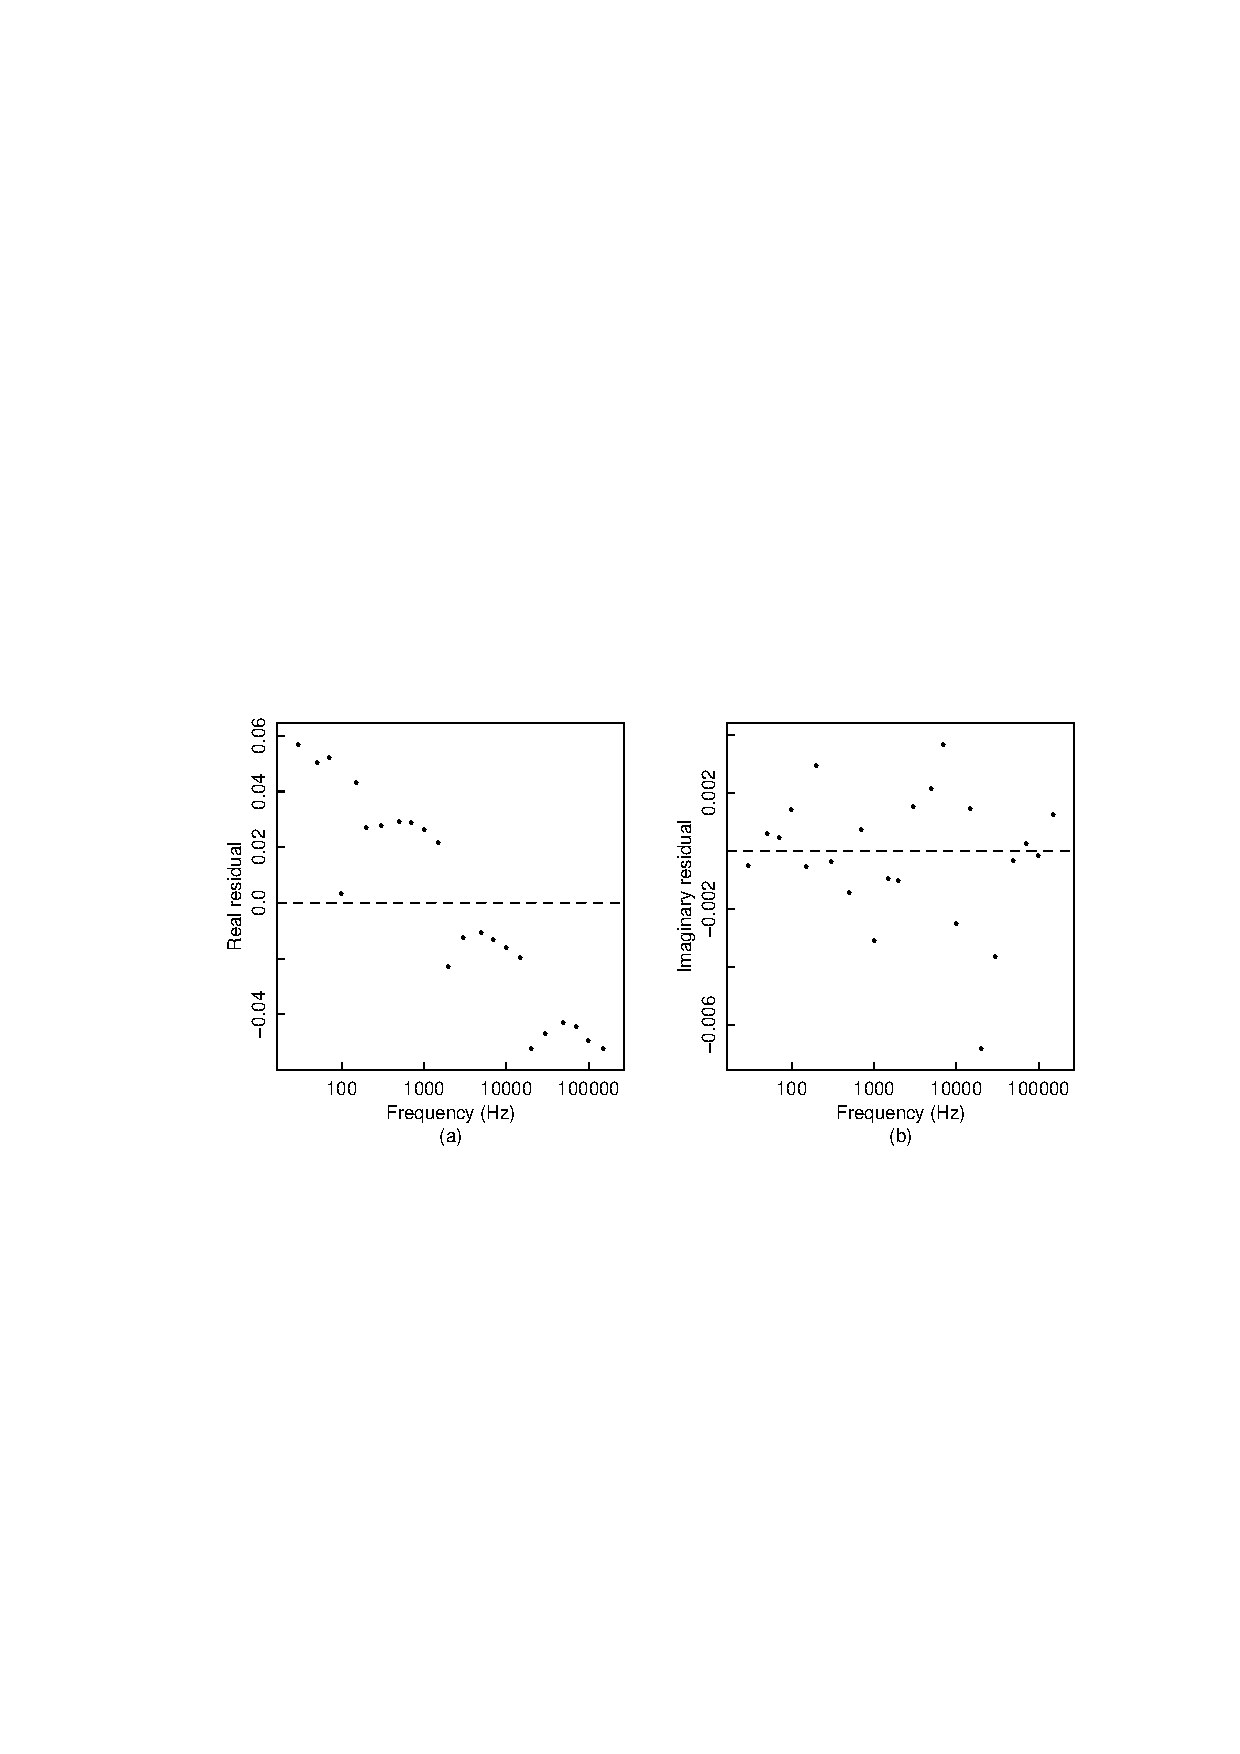
\includegraphics{4PMMAres1}}%,height=2.25in}}
  \caption{\label{fig:PMMAres1}
  Residuals from the initial fit to the s-PMMA data.
  }
\end{figure}
The imaginary residuals are quite well behaved, but the
real residuals are grouped and have a strong trend
with frequency.

As discussed in \citeasnoun{havr:watt:1987},
%\glossary{ Havriliak, S.Jr.}
%\glossary{ Watts, D.G.}
this behavior can be explained by considering the way in
which the frequencies are set in an experiment.
When the frequency of an oscillator is made to cover an
extremely large range (in this example, from 30 to
150000 Hz), it is done by manipulating two dials, a {\em units\/}
dial which covers a range of, say, 2 to 20,
and a {\em decade\/} dial which changes the frequency by
multiples of 10.
Thus, to set the frequency to 150 Hz, the
operator would set the units dial to 15 and the
decade dial to $\times 10$; and to set the frequency to 30000
Hz, the operator would set the units dial to 3 and the
decade dial to $\times 10000$.
In this experiment, the capacitance of
the polymer sample was apparently large enough to affect the
frequency of the oscillator, so that the actual frequency
delivered was not that indicated on the dials.
At high
frequencies the fitted values were too large, and at low
frequencies the fitted values were too small, suggesting
that the indicated frequencies were below the actual, with
the discrepancy (indicated -- actual) increasing with each decade
increase.

A decade correction was therefore made to the indicated
frequencies so that when the decade was increased, the
frequency was multiplied by $10\times K$.
Assuming the
first decade was correct, the second decade would have
actual frequencies of $K \times$ the indicated values, the
third decade $K^{2\times} $ the indicated values, and so
on.
Rather than incorporate the decade factor $K$ as a
parameter in the model, we performed a search by selecting
values for $K$, modifying the indicated frequencies,
fitting the model and examining the residuals, and choosing
that value of $K$ which gave the best behaved residuals.
For this data set, a decade correction of $K = 1.25 $ was
found.

The convergence output for the decade-corrected data is
given in
Table~\ref{tbl:4.3}.
\begin{table}
  \caption{\label{tbl:4.3}
  Parameter summary for the decade-corrected s-PMMA data
  }
  \begin{center}
    \begin{tabular}{cllrrrrr}\hline
      \multicolumn{1}{c}{Parameter} & \multicolumn{1}{c}{Estimate} &
      \multicolumn{1}{c}{Approx.} & \multicolumn{5}{c}{Approximate}\\
      && \multicolumn{1}{c}{Std.Error} &
      \multicolumn{5}{c}{Correlation Matrix}\\ \hline
      $\epsilon_{0}$&4.400&0.007&1.00\\
      $\epsilon_{\infty}$&2.447&0.013&0.58&1.00\\
      $\ln f_{0}$&8.228&0.091&0.68&0.84&1.00\\
      $\alpha$&0.486&0.008&--\/0.86&--\/0.68&--\/0.91&1.00\\
      $\beta$&0.571&0.026&0.76&0.85&0.99&--\/0.95&1.00\\ \hline
    \end{tabular}
  \end{center}
\end{table}
The major changes were a reduction in the determinant and in
the variance estimate of the real residuals by
a factor of about 10.
The residuals for the real and imaginary components are
plotted versus frequency in
Figure~\ref{fig:PMMAres2},
\begin{figure}
  \centerline{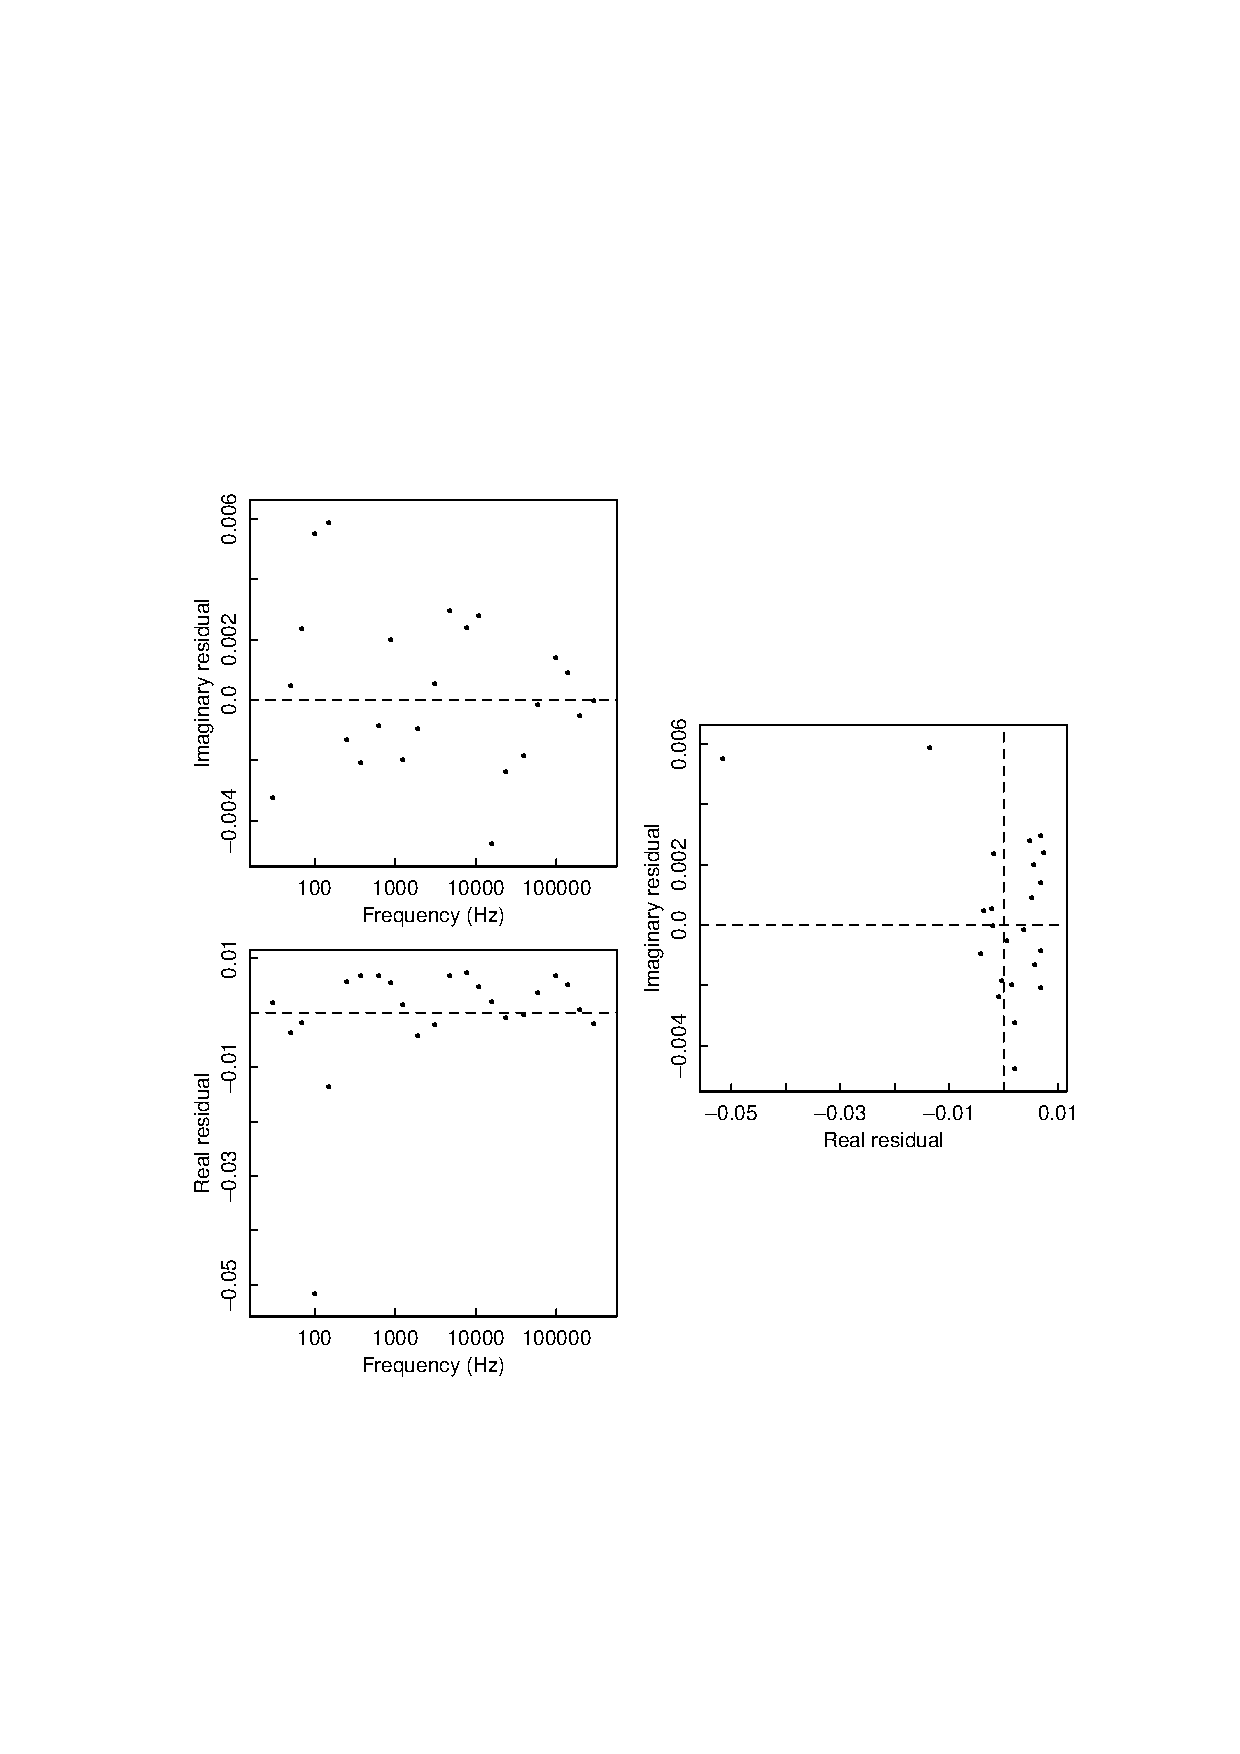
\includegraphics{4PMMAres2}}%,height=4.5in}}
  \caption{\label{fig:PMMAres2}
  Residuals from the fit to the decade-corrected s-PMMA data.
  }
\end{figure}
from which it can be seen that the imaginary residuals are
very well behaved, with perhaps two or three outliers.
The real residuals are much better behaved now, with no trend.
There is, however, one obvious outlier and one other
possible outlier.
Plotting the imaginary residuals versus the real residuals
more clearly discloses two outliers.
Since the residuals are bad in both the real and imaginary components,
we simply delete these two cases.
If only one residual were bad, we could treat the
observation which gave rise to the bad residual as missing, and
proceed as in Section 4.4.

Analysis of the decade-corrected and edited data set produced
the results in
Table~\ref{tbl:4.4}.
\begin{table}
  \caption{\label{tbl:4.4}
  Parameter summary for the decade-corrected and edited s-PMMA data}
  \begin{center}
    \begin{tabular}{cccrrrrr}\hline
      \multicolumn{1}{c}{Parameter} & \multicolumn{1}{c}{Estimate} &
      \multicolumn{1}{c}{Approx.} & \multicolumn{5}{c}{Approximate}\\
      && \multicolumn{1}{c}{Std.Error} &
      \multicolumn{5}{c}{Correlation Matrix}\\ \hline 
      $\epsilon_{0}$&4.398&0.006&1.00\\
      $\epsilon_{\infty}$&2.451&0.010&0.53&1.00\\
      $\ln f_{0}$&8.245&0.074&0.63&0.91&1.00\\
      $\alpha$&0.487&0.007&--\/0.86&--\/0.75&--\/0.90&1.00\\
      $\beta$&0.571&0.021&0.74&0.91&0.98&--\/0.95&1.00\\
    \end{tabular}
  \end{center}
\end{table}
Removing the two unusual cases reduced the parameter and
variable variances, but the parameter estimates were not
materially affected.
The residuals from this fit are very well behaved, as can
be seen from Figure~\ref{fig:PMMAres3}.
\begin{figure}
  \centerline{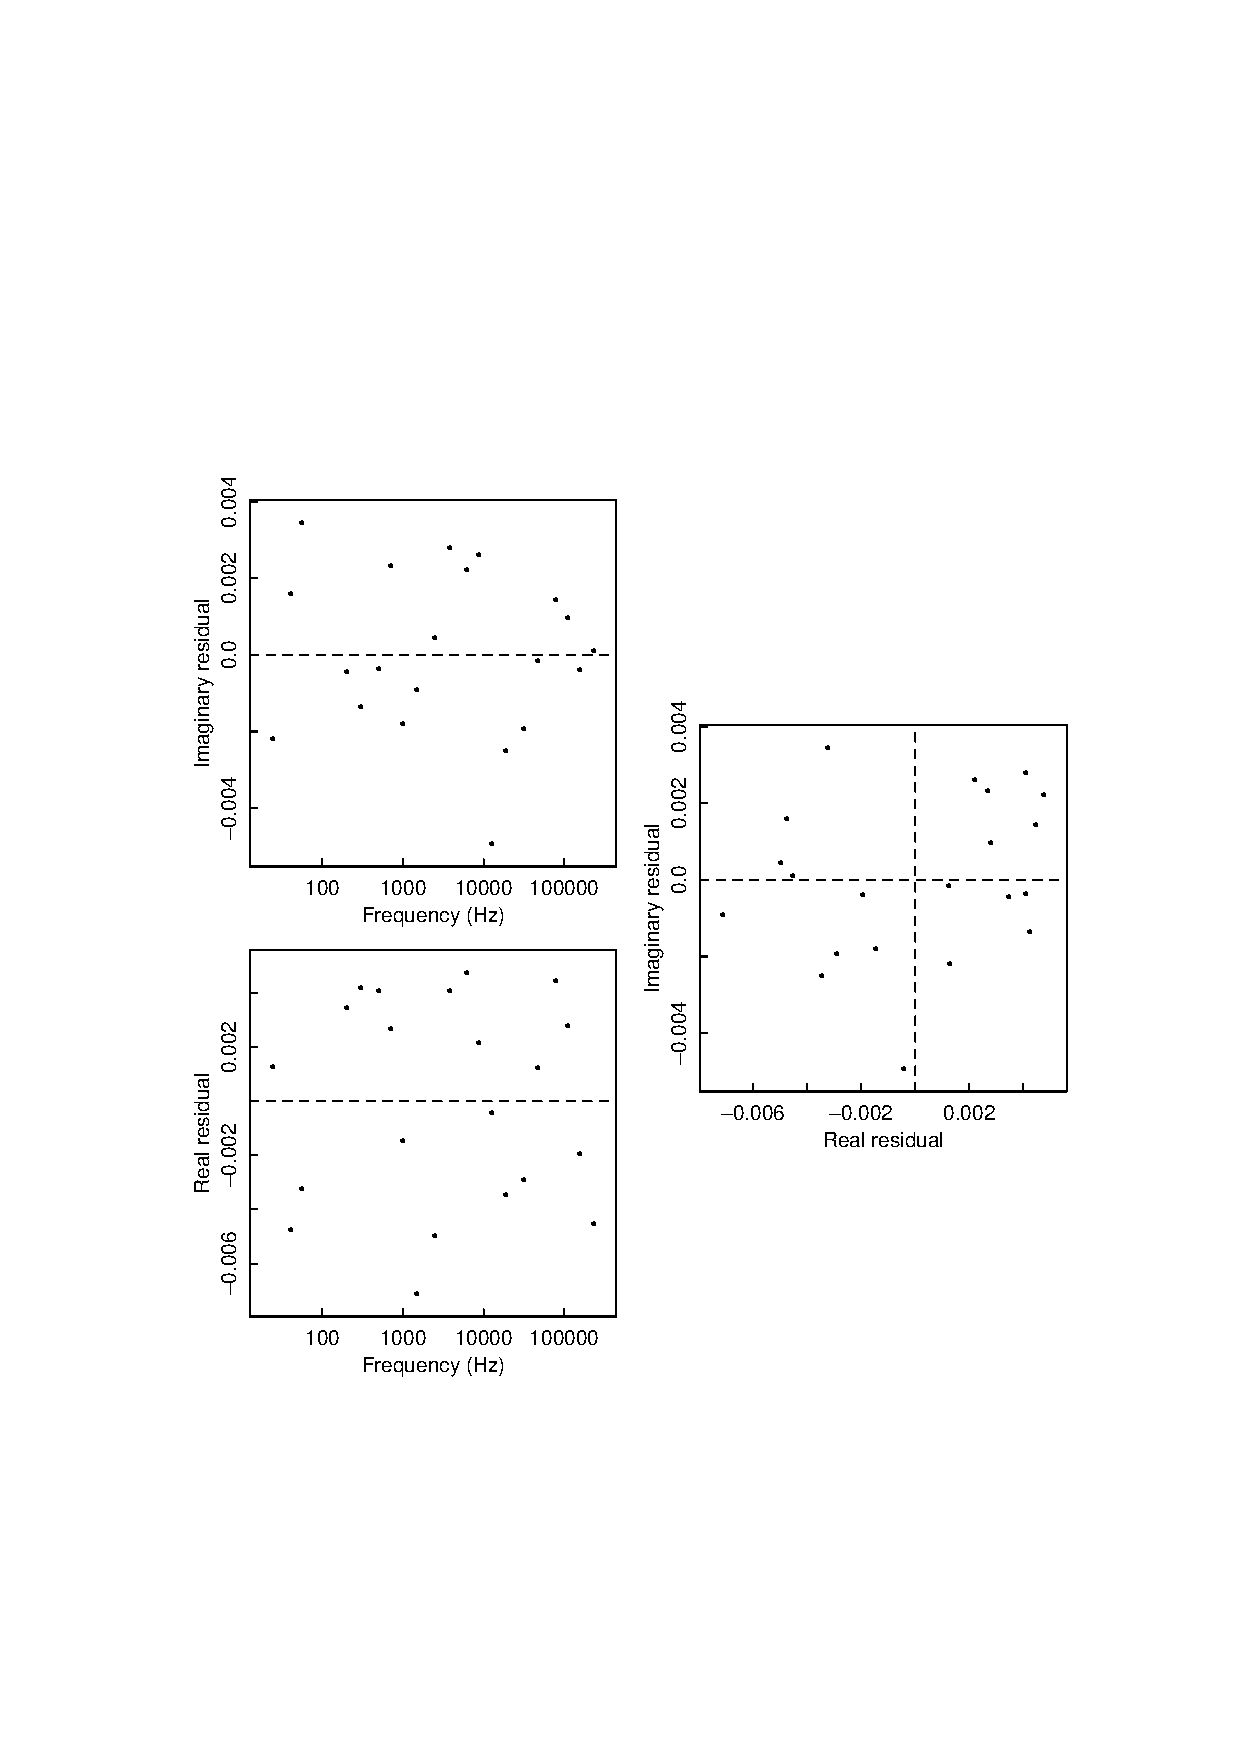
\includegraphics{4PMMAres3}}%,height=4.5in}}
  \caption{\label{fig:PMMAres3}
  Residuals from the fit to the decade-corrected and edited s-PMMA data.}
\end{figure}

We also analyzed the data by estimating $K$ rather than
obtaining it from a search.
The optimum value was $\hat K=1.24$;
the other parameter estimates and their approximate standard errors
changed slightly.
\end{example}

\begin{example}\label{pin:3}

The starting values in Example $\alpha$-Pinene 2 were used together with
the techniques described in
Chapter 5 for obtaining the expectation function and derivatives, and
convergence was obtained for the five response data set as shown
in Table~\ref{tbl:4.5}.
\begin{table}
  \caption{\label{tbl:4.5}
  Parameter summary for the -pinene data using five responses}
  \begin{center}
    \begin{tabular}{ccrrrrrrrr}\hline
      \multicolumn{2}{c}{Parameter} & \multicolumn{1}{c}{$\theta$} &
      \multicolumn{7}{c}{Logarithm Scale}\\
      \multicolumn{1}{c}{From} &\multicolumn{1}{c}{To} &
      \multicolumn{1}{c}{$( 10^{-5} )$}  & \multicolumn{1}{c}{$\phi$}
      & \multicolumn{1}{c}{Std.Error} & \multicolumn{5}{c}{Correlation}\\ \hline
      1&2&3.74&--10.19&0.085&1.00\\
      1&3&1.95&--10.85&0.073&0.84&1.00\\
      3&4&1.65&--11.01&0.104&--\/0.20&--\/0.41&1.00\\
      3&5&27.01&--8.217&0.128&0.00&--\/0.00&0.85&1.00\\
      5&3&2.61&--10.55&0.195&0.68&0.78&--\/0.01&0.40&1.00\\ \hline
    \end{tabular}
  \end{center}
\end{table}
In Figure~\ref{fig:BHME5pred}
\begin{figure}
  \centerline{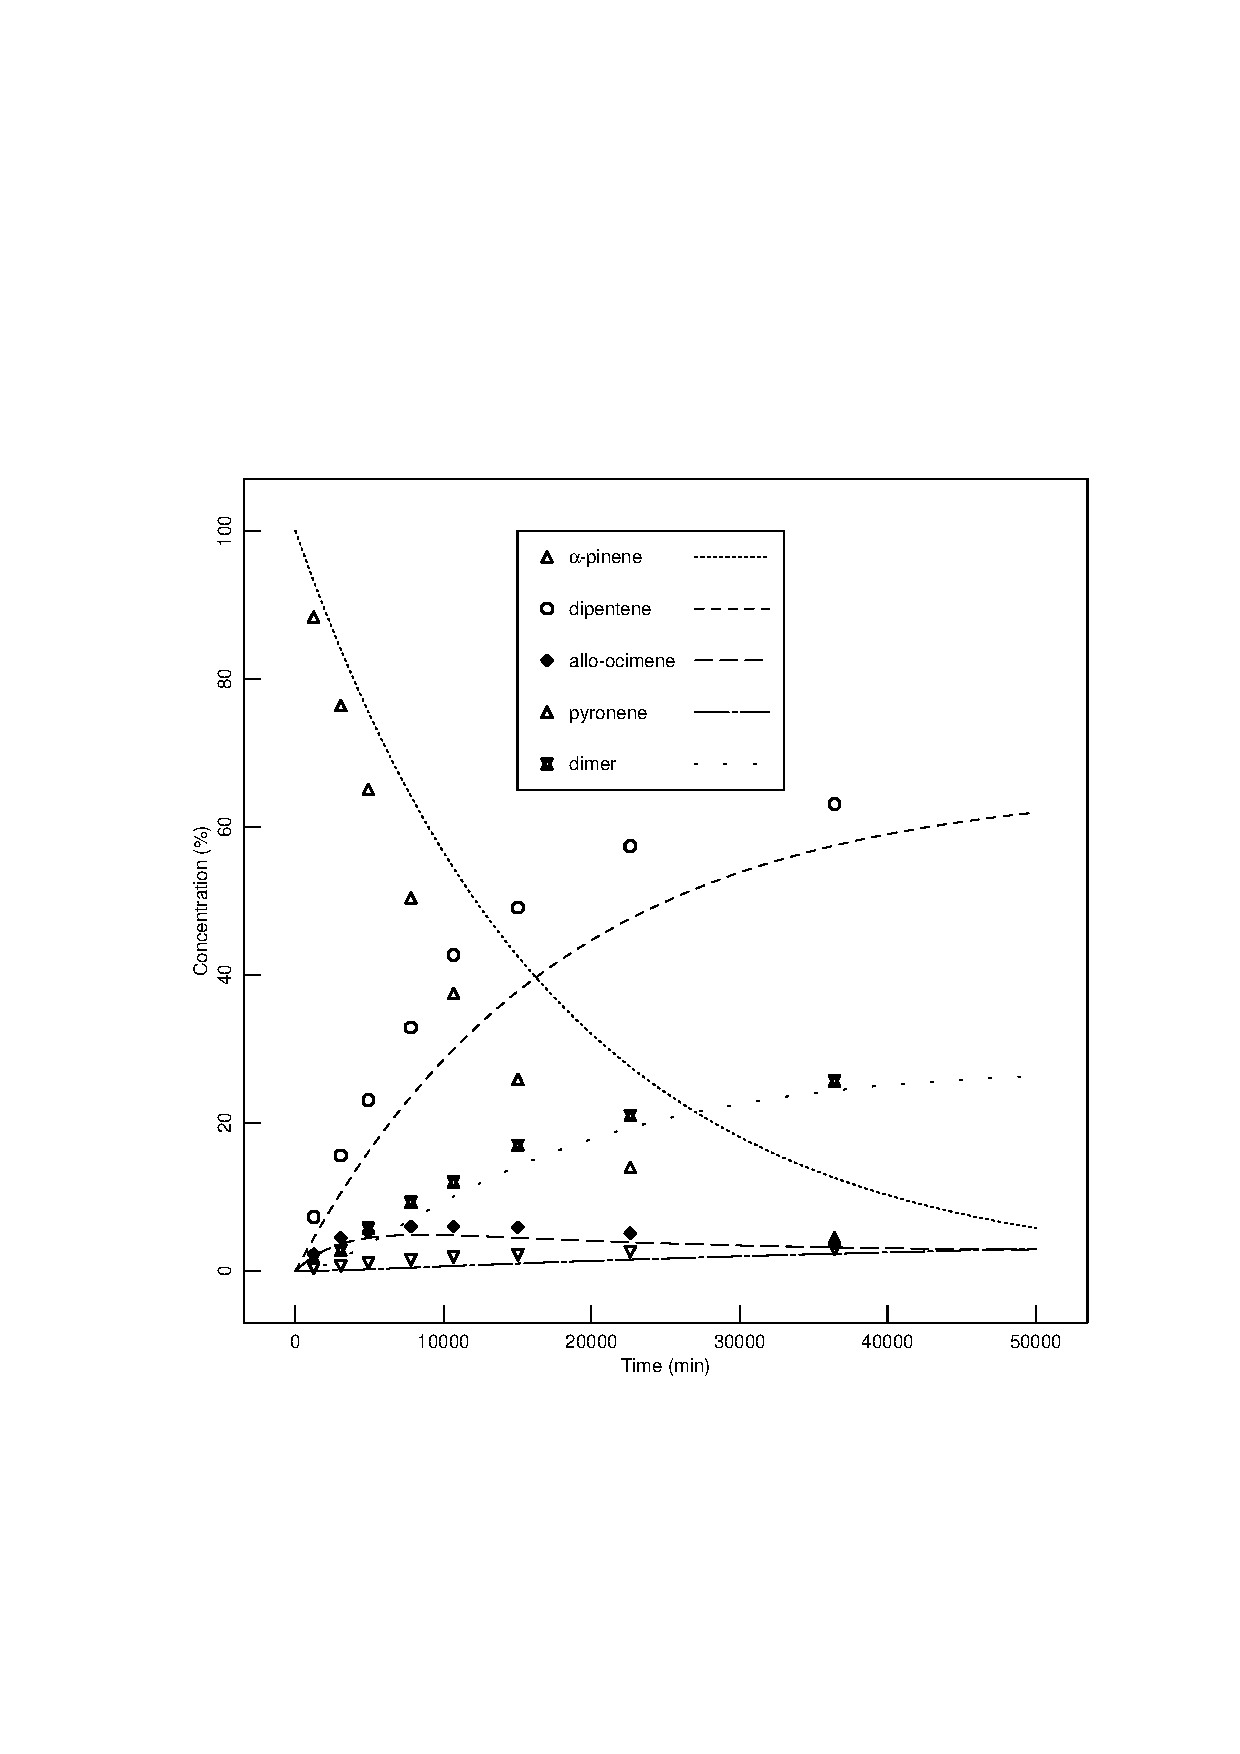
\includegraphics{4BHME5pred}}%,height=4.5in}}
  \caption{\label{fig:BHME5pred}
  Observed values and the predicted curves obtained by fitting five
  responses to the $\alpha$-pinene data}
\end{figure}
we show a plot of the data and the fitted
responses.
The fitted curves do not follow the data very well, suggesting
that convergence to a spurious optimum has occurred.
As will be shown in the next section, this has occurred
because there are dependencies in the data.
\end{example}

\subsection{Dependencies Among Responses}
\index{dependencies!in multiresponse data}
\index{multiresponse estimation!dependencies in data}

Convergence to a spurious optimum due to dependencies in the response data
\index{convergence!to spurious optimum}
is an important problem which can easily arise in multiresponse
estimation, but which can not happen in uniresponse estimation.
Data dependencies can occur, for example, because the responses are
\index{dependencies!in multiresponse estimation}
constrained through mass balances or because one or more responses
are not measured but are imputed from other measured responses.
If dependencies occur in the data or in the expected responses,
then the estimation procedure must be modified so as to avoid
convergence to spurious optima
\cite{box:hunt:macg:erja:1973,mcle:prit:baco:down:1979}.
%\glossary{ Box, G.E.P.}
%\glossary{ Hunter, W.G.}
%\glossary{ MacGregor, J.M.}
%\glossary{ Erjavec, J.}
%\glossary{ McLean, D.D.}
%\glossary{ Pritchard, D.J.}
%\glossary{ Bacon, D.W.}
%\glossary{ Downie, J.}

To detect dependencies in a multiresponse data set,
\citeasnoun{box:hunt:macg:erja:1973}
%\glossary{ Box, G.E.P.}
%\glossary{ Hunter, W.G.}
%\glossary{ MacGregor, J.M.}
%\glossary{ Erjavec, J.}
used an eigenvalue analysis of the
\index{eigenvalue!analysis of centered data matrix}
inner product of the centered data matrix,
\index{matrix!centered data}
$( \bar \bY ) \trans ( \bar \bY )$,
where $\bar \bY$ is the matrix of response averages
obtained by replacing each column of $\bY$ by the average of the column.
They then compared the eigenvalues with an estimate of the roundoff
sum of squares,
$( N-1 ) u^2 / 12 $,
where $u$ is the rounding unit of the data.
Any eigenvalues which were of the same magnitude as the roundoff sum
of squares were
assumed to be associated with linear dependencies in the data.

This approach can reveal singularities
\index{singular!data matrix}
due to conditions that cause a linear combination of the
responses from all cases to be a constant (for example, a mass balance),
but, as described in \citeasnoun{mcle:prit:baco:down:1979}
%\glossary{ McLean, D.D.}
%\glossary{ Pritchard, D.J.}
%\glossary{ Bacon, D.W.}
%\glossary{ Downie, J.}
analysis of the centered {\em data\/} matrix
can fail to detect singularities in the {\em residual\/}
matrix, and hence
\index{singular!residual matrix}
\index{residual!matrix}
\index{matrix!residual}
\index{matrix!singular}
one may still be trying to converge with a ``defective''
data set.
As was also pointed out by these authors, in certain circumstances
linear dependencies among the data need not cause singularities in
the residual matrix $\bZ ( \btheta ) $,
so removal of singularities detected through analysis of the centered data
matrix can cause unnecessary loss of precision in the parameter estimates.
Therefore, it is necessary to search for singularities in
both the centered data matrix and the residual matrix.

As an example where there can be singularities in
$\bZ$ but no singularities in $ \bar \bY $, following
\citeasnoun{mcle:prit:baco:down:1979}, we consider a chemical reaction
%\glossary{ McLean, D.D.}
%\glossary{ Pritchard, D.J.}
%\glossary{ Bacon, D.W.}
%\glossary{ Downie, J.}
in which two responses are measured.
The two responses are normalized
so that the total for the $n$th case is $\gamma_n^{0}$,
the initial concentration of the first chemical.
Unless the initial concentrations are all the same, the matrix
$ \bY - \bar \bY $ will not be singular.
However, if the reaction follows first order kinetics so that
$f_{n1}=\gamma_n^0 e^{{-} \theta t_n }$ and
$f_{n2}=\gamma_n^0 ( 1 - e^{ - \theta t_n } )$,
then the residual matrix $\bZ$ with $n$th row
$$
( z_{n1} , z_{n2} ) =
( y_{n1} - f_{n1} ,  y_{n2} - f_{n2} )
$$
involves the linear dependency $z_{n1}+z_{n2}=0$
for all $n$, and the residual matrix is singular.
It would be futile, therefore, to try to estimate the parameter $\btheta$
using a multiresponse estimation criterion.

As an example where there can be singularities in
$ \bY - \bar \bY $ but no singularities in $\bZ$,
suppose that in the example above, the
two responses are obtained from chromatograph area
fractions, so the measurement for $y_{n1} $ is
$$
y_{n1} = a_1 +
b_1 \left({{\rm area}_{n1} \over {\rm area}_{n1+{\rm }} area_{n2}}
\right)
$$
and that for $ y_{n2} $ is
$$
y_{n2} = a_2 +
b_2 \left({{\rm area}_{n2} \over {\rm area}_{n1+{\rm }} area_{n2}}
\right)
$$
where $a_{1}$, $b_{1}$, $a_{2}$, and $b_{2}$ are calibration
constants.
Then a linear dependency will exist in the data of the form
$ b_2  y_{n1}+b_1 y_{n2} = \mbox{\rm constant}$ for all n, and so $  \bY - \bar \bY  $ will be singular.
However, unless for every case
$$
 \gamma_n^0 \left[ b_1 + ( b_2 - b_1 )
e^{ - \theta t_n } \right] =
a_2 b_1 + a_1 b_2 + b_1 b_2
$$
the residual matrix will not be singular because of the linear
dependence in the data.

Singularities in $ \bY - \bar \bY $ and in $\bZ$ can be detected by
performing an eigenvalue--eigenvector decomposition of the inner
product, as proposed by
\citeasnoun{box:hunt:macg:erja:1973},
%\glossary{ Box, G.E.P.}
%\glossary{ Hunter, W.G.}
%\glossary{ MacGregor, J.M.}
%\glossary{ Erjavec, J.}
but we prefer to arrange the rounding units in the columns of $\bY$ to
be approximately equal and then take singular value decompositions of
\index{singular value decomposition}
$ \bar \bY $ and $\bZ$ \cite[Chapter 11]{dong:bunc:mole:stew:1979}.
%\glossary{ Dongerra, J.J.}
%\glossary{ Bunch, J.R.}
%\glossary{ Moler, C.B.}
%\glossary{Stewart, G.W.}
As explained there, singular values on the order of
the rounding unit indicate singularity and should prompt the
analyst to search for dependencies in the data.

A singular value decomposition of the centered data matrix, and
of the residual matrix using the initial parameter values,
should be done at the beginning of the analysis so as to avoid
unnecessary calculations caused by dealing with a defective
data set which involves linear dependencies.
If small singular values are obtained, the corresponding singular
vectors should be examined to reveal what is causing the
dependencies.
If the dependency can be explained (e.g., a mass balance, or a response
has been imputed from other measured responses) and the offending
responses identified, they should be removed and a multiresponse
analysis performed on the reduced data set.
If a dependency can not be explained, then the multiresponse analysis
should be modified to take account of the dependency as described
in Section 4.3.4.
The residual matrix at the converged parameter values
should also be analyzed for singular values
so as to detect possible dependencies in the residuals.
Further comments on detecting and eliminating linear
dependencies are given in
\citeasnoun{mcle:prit:baco:down:1979}.
%\glossary{ McLean, D.D.}
%\glossary{ Pritchard, D.J.}
%\glossary{ Bacon, D.W.}
%\glossary{ Downie, J.}

\begin{example}\label{spmma:4}
For the decade-corrected and edited s-PMMA data, the singular
values of the centered data matrix
are 0.278 and 2.161, and since
the rounding units in the data are both 0.001,
neither of these singular values is small
enough to suggest a linear dependency.
The singular values of the residual matrix at the converged values
are 0.009 and 0.017 and neither of these is small enough to cause
concern.
\end{example}

\begin{example}\label{pin:4}
The centered data matrix for the $\alpha$-pinene data, has the
singular value decomposition
%Singular value:0.04:0.13:1.10:5.08:98.30
%_
%Singular vectors:\-\^0.17:0.48:\-\^0.30:0.06:\-\^0.81
%\^:\-\^0.21:0.49:\-\^0.61:\-\^0.22:0.54
%\^:\-\^0.16:0.43:0.64:\-\^0.61:0.01
%\^:0.93:0.36:\-\^0.01:0.00:0.02
%\^:\-\^0.19:0.46:0.36:0.76:0.23
%.TE
which clearly indicates dependencies in the data because
the two small singular values are of the same magnitude as
the rounding unit in the data (0.1, see Appendix 1, Section A1.6).

The residual matrix at the starting estimates has
the singular value decomposition
%Singular value:0.06:0.14:0.46:1.63:42.70
%_
%Singular vectors:0.34:\-\^0.30:\-\^0.28:0.26:0.81
%\^:0.39:\-\^0.26:\-\^0.39:0.55:\-\^0.57
%\^:0.60:\-\^0.27:0.75:\-\^0.08:\-\^0.07
%\^:\-\^0.50:\-\^0.86:0.08:\-\^0.05:\-\^0.06
%\^:0.36:\-\^0.20:\-\^0.45:\-\^0.79:\-\^0.12
which also reveals two dependencies.

As noted by \citeasnoun{box:hunt:macg:erja:1973}, from careful reading of the
%\glossary{ Box, G.E.P.}
%\glossary{ Hunter, W.G.}
%\glossary{ MacGregor, J.M.}
%\glossary{ Erjavec, J.}
paper by \citeasnoun{fugu:hawk:1947}, the response $y_4 $ was
%\glossary{ Fuguitt, R.E.}
%\glossary{ Hawkins, J.E.}
not in fact measured, but was imputed as 3\% of the
amount of converted $y_{1}$, i.e.,
$y_4=$ $0.03 ( 100 - y_1 )$.
The first singular vector of the centered data matrix reflects this
dependency and so
the imputed data for $y_4 $ should not be used in estimation.
The second singular vector, consisting of almost equal entries,
reflects a mass balance dependency, i.e., the data must sum to
100\%.
This occurs because the system is a conservative one, as can
easily be seen, since all the columns of the system matrix $\bA$
sum to zero.
The singular vectors of the residual matrix do not reflect these
dependencies, so that while the singular value decomposition of $\bZ$
does suggest that there are dependencies, it does not reveal their
nature.

Because there are two small singular values, suggesting two
linear dependencies in the data, only three responses
should be retained for parameter estimation.
\end{example}

When linear dependencies are found, the problem of
choosing an appropriate subset of the responses must be addressed.
One approach is to retain those responses which the researcher
thinks are most reliable.
It may not be possible to select the responses on this basis, however,
and so we follow \citeasnoun{box:hunt:macg:erja:1973} and use
%\glossary{ Box, G.E.P.}
%\glossary{ Hunter, W.G.}
%\glossary{ MacGregor, J.M.}
%\glossary{ Erjavec, J.}
a linear combination of the responses instead.
In either situation, it would be helpful to have a procedure for
estimating parameters in the presence of dependencies.
Accordingly, in the following section we describe a procedure for
estimating parameters in the presence of linear dependencies.

\subsection{Linear Combinations of Responses}
\index{dependencies!in multiresponse estimation}

Suppose there are $d$ linear dependencies, and there are no missing
values in the data matrix.
To deal with linear dependencies,
we generate an $N \times ( M - d )$ reduced residual matrix
$\bZ \bB$ by combining the $d$ linear dependency
vectors into an $M \times d$ dependency matrix $\bD$, performing a $QR$
decomposition
on $\bD$, and letting the rotation matrix $\bB$ be the $ M-d $
columns of $\bQ$ which are orthogonal to the dependency vectors.

\begin{example}\label{pin:5}
For the $\alpha$-pinene data, we have decided that response 4
should not be used in estimation, and that there is a mass
balance relation in the data.
The dependency matrix is therefore
$$
\bD = \left[ \matrix {
\matrix { 0 \cr 0 \cr 0 \cr 1 \cr 0 }
\matrix { 1 \cr 1 \cr 1 \cr 1 \cr 1 }
}\right]
$$
Performing a $QR$ decomposition produces $\bB$ as the last three
columns of $\bQ$.
Again, as discussed in Appendix 2, although $\bQ$ is required to obtain
$\bB$, $\bQ$ is not explicitly formed; a product
such as $\bZ_{(p)} \bB$ is formed by applying Householder
transformations to $\bZ_{(p)} \trans $, retaining the last $M - d$
rows to give $( \bZ_{(p)} \bB ) \trans$, and then transposing the result.
\end{example}

To minimize $ | ( \bZ \bB ) \trans ( \bZ \bB ) |$ using the generalized
Gauss--Newton method of Section 4.2, we need $( \bZ \bB )_{(p)} $.
This is easily obtained because $\bB$ is independent of $\btheta$, and so
$$
( \bZ \bB )_{(p)} = \bZ_{(p)} \bB
$$
Thus, the terms in the determinant, the gradient and the approximate
Hessian for the reduced data set can be calculated by simply using
$ \bZ $ and $ \bZ_{(p)} , p = 1 ,\ldots, P$.

\begin{example}\label{pin:5a}
Using the starting values from Example $\alpha$-Pinene \ref{pin:3} and
three (rotated) responses, we obtained the results in
Table~\ref{tbl:4.6}.
\begin{table}
  \caption{\label{tbl:4.6}
  Parameter summary for the $\alpha$-pinene data using three rotated
  responses}
%c s c c s s s s s s
%c s c c s s s s s s
%c1 c c c1 c c s s s s
%c1 c n n1 n n1 n1 n1 n1 n.
%\_
%Parameter:$\theta$:Logarithm Scale
%From:To:$( 10^{-5} )$:$\phi$:Std.Error:Correlation
%\_
%1:2:5.94:--9.731:0.021:1.00
%1:3:2.86:--10.47:0.042:--\/0.20:1.00
%3:4:0.453:--12.31:3.92:--\/0.37:0.91:1.00
%3:5:31.12:--8.072:0.124:--\/0.22:0.51:0.45:1.00
%5:3:5.79:--9.757:0.21:0.10:0.16:0.16:0.78:1.00
%\_
\end{table}
The overlay plot of the data and fitted curves in
Figure~\ref{fig:BHME3pred}
  \begin{figure}
    \centerline{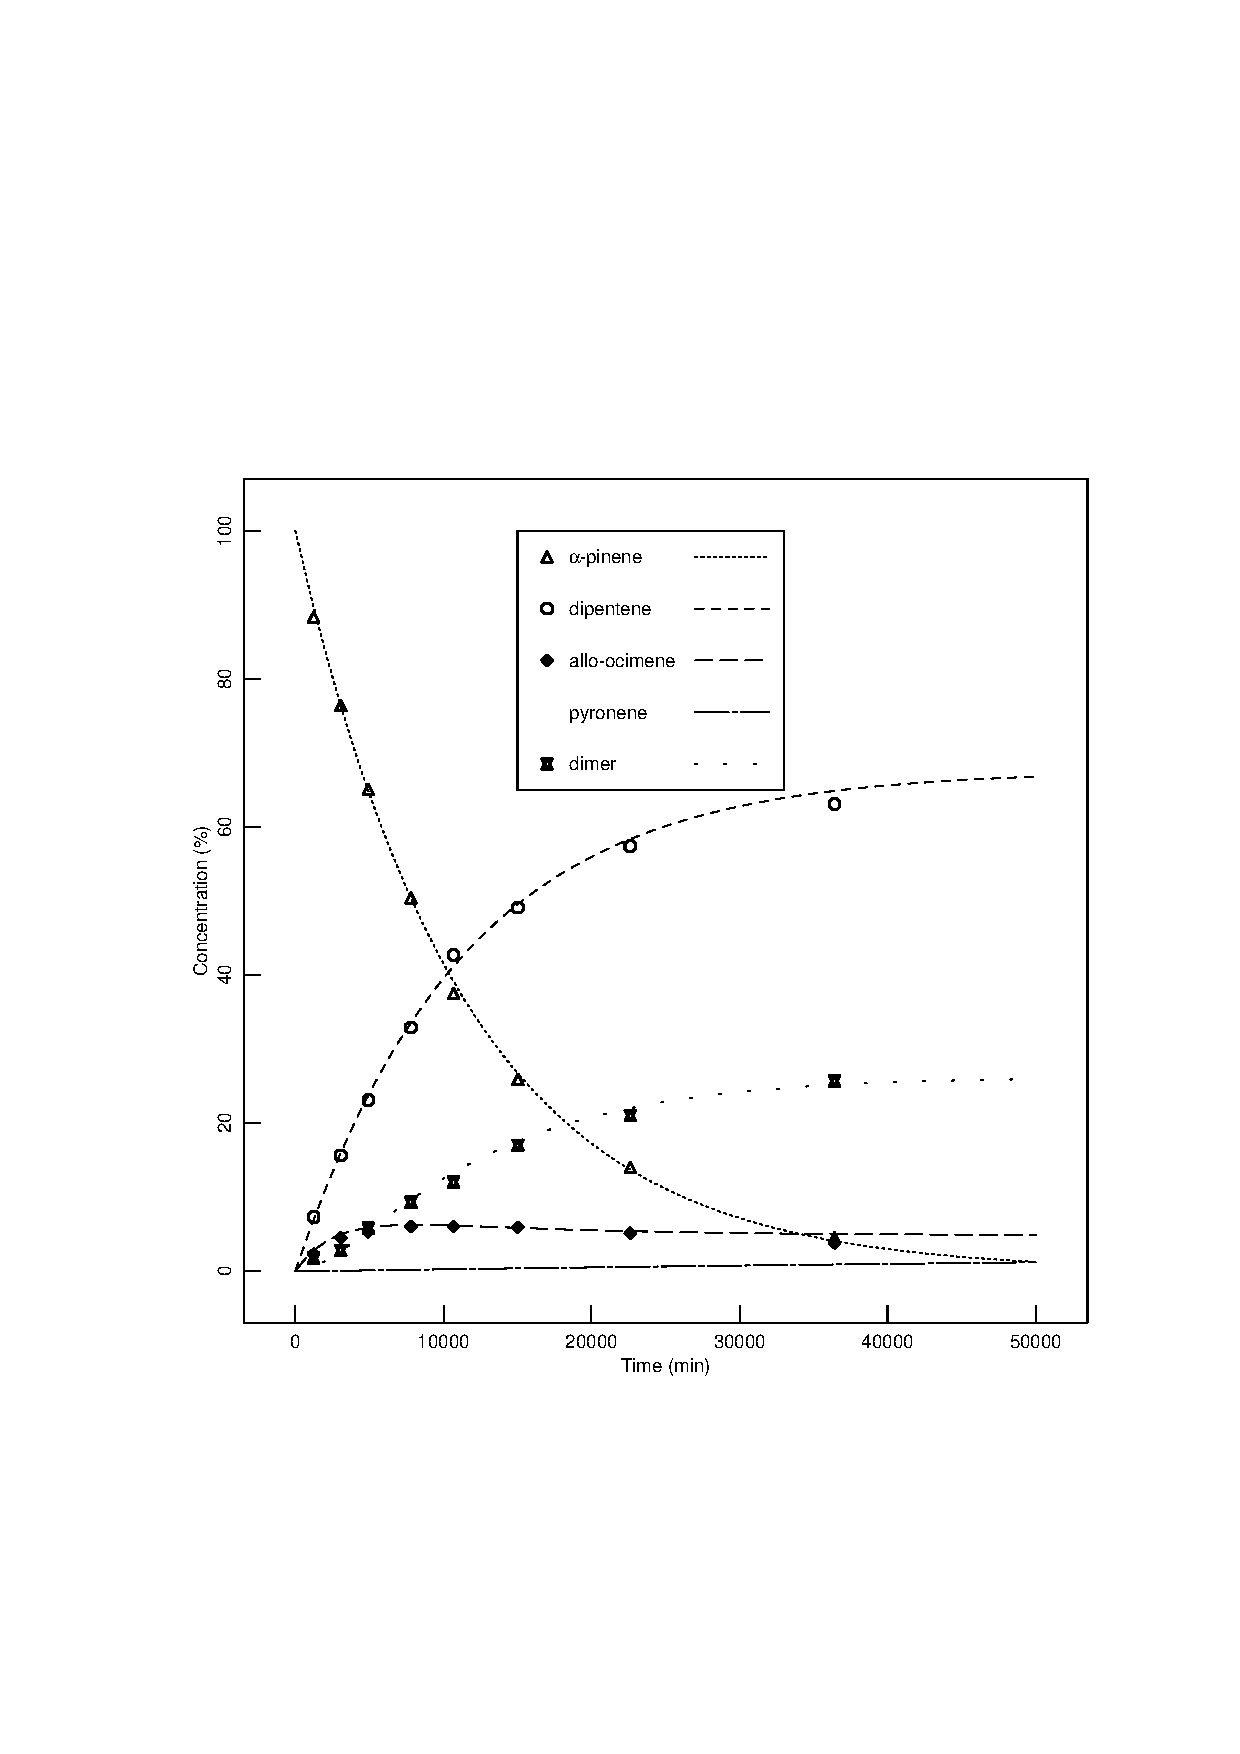
\includegraphics{4BHME3pred}}%,height=4.5in}}
    \caption{\label{fig:BHME3pred}
    Observed values and the predicted curves obtained by fitting three
    rotated responses to the $\alpha$-pinene data.
    }
  \end{figure}
gives no evidence of inadequacy of the fitted model.
However, the residuals, shown in Figure~\ref{fig:BHME3res},
  \begin{figure}
    \centerline{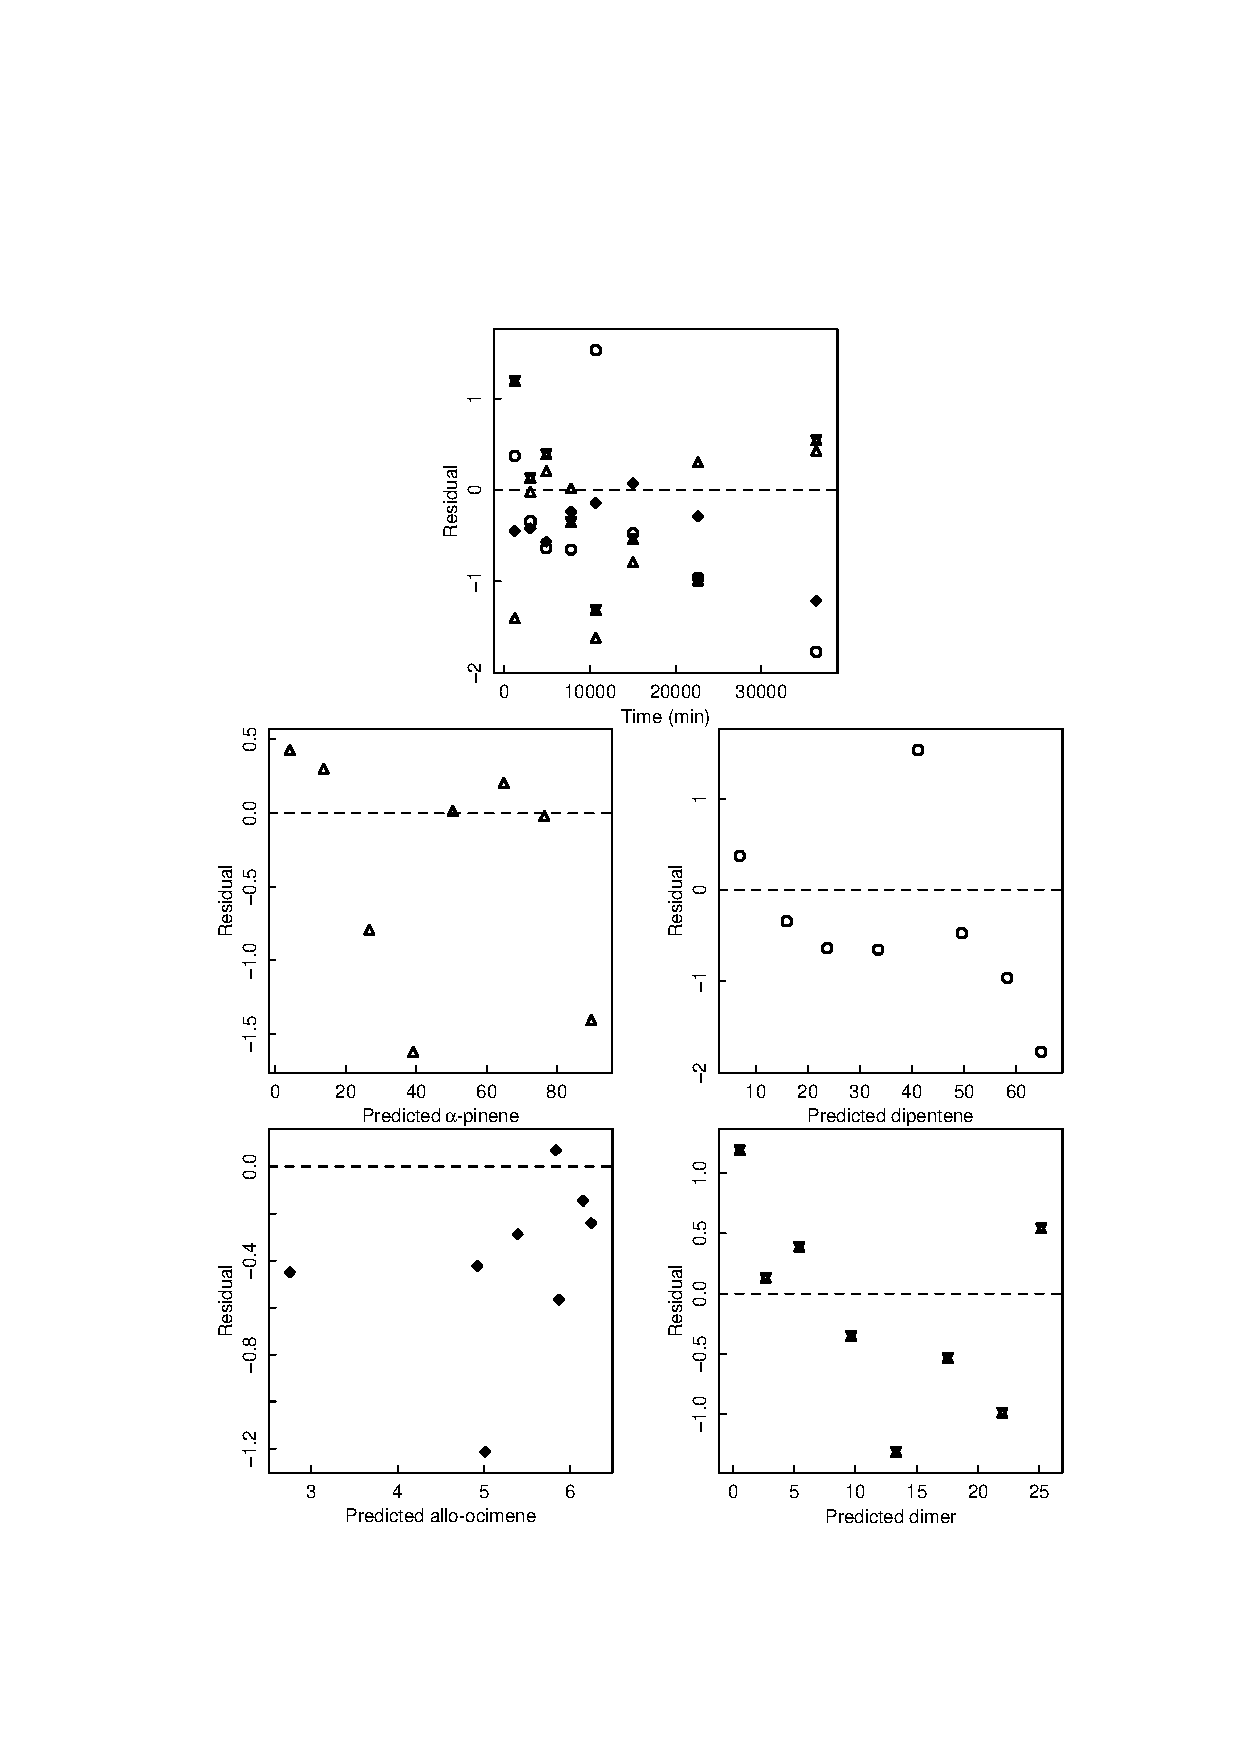
\includegraphics{4BHME3res}}%,width=\textwidth}}
    \caption{\label{fig:BHME3res}
    Residuals from the three rotated response fit to the $\alpha$-pinene
    data plotted versus time and versus predicted response.
    }
  \end{figure}
are not well behaved, with a large negative residual for response 3 and
a trend and a large positive residual for response 2.
There is also a preponderance of negative residuals.
Also the approximate confidence limits on $\phi_{3}$ are
very wide, suggesting that it is badly estimated and that $\theta_{3}$
could be zero.
We temporarily ignore the defective residuals, and try to see if a
simpler model would be adequate.
\end{example}

Linear combinations of responses can be used to check for consistency of
information by analyzing subsets of the responses, as suggested in
\citeasnoun{box:drap:1965}.
%\glossary{ Box, G.E.P.}
%\glossary{ Draper, N.R.}
We simply let $\bB$ be the matrix derived from an identity
matrix by deleting columns corresponding to the unused responses.

\begin{example}\label{pin:5b}
Suppose we wished to estimate the
parameters using only the responses $y_{1}$, $y_{2}$, and $y_{5}$.
Then we would use as the rotation matrix
$$
\bB = \left[ \matrix {
\matrix { 1 \cr 0 \cr 0 \cr 0 \cr 0 }
\matrix { 0 \cr 1 \cr 0 \cr 0 \cr 0 }
\matrix { 0 \cr 0 \cr 0 \cr 0 \cr 1 }
}\right]
$$
\end{example}

\subsection{Comparing Models}

Nested models can be compared using an
\index{model!nested}
``extra determinant''
\index{extra determinant!test for nested models}
\index{nested model!extra determinant test}
analysis in the same way that uniresponse nested models were compared
using an extra sum of squares analysis (Section 3.10).
That is, we compare the ratio of the change in the determinant divided
by the change in the degrees of freedom with the scaled determinant
for the complete model as in (\ref{eqn:Fregion}).

\begin{example}\label{pin:6}
The model for the $\alpha$-pinene reaction includes a path from species
3 to species 4, but as seen in Example $\alpha$-Pinene~\ref{pin:5},
the logarithm of the rate constant associated with that path has a
large standard error, suggesting that this path could be eliminated.
Fitting the data without this path, but still retaining only three
(rotated) responses, gives the results in
Table~\ref{tbl:4.7}.
\begin{table}
  \begin{center}
    \begin{tabular}{ccrrrrrrr}\hline
      \multicolumn{2}{c}{Parameter} & \multicolumn{1}{c}{$\theta$} &
      \multicolumn{6}{c}{Logarithm Scale}\\
      \multicolumn{1}{c}{From} &\multicolumn{1}{c}{To} &
      \multicolumn{1}{c}{$( 10^{-5} )$}  & \multicolumn{1}{c}{$\phi$}
      & \multicolumn{1}{c}{Std.Error} & \multicolumn{4}{c}{Correlation}\\ \hline
      1&2&5.94&--9.73&0.018&1.00\\
      1&3&2.82&--11.28&0.016&0.44&1.00\\
      3&5&30.75&--8.09&0.093&--\/0.07&0.26&1.00\\
      5&3&5.72&--9.77&0.182&0.16&0.05&0.81&1.00\\ \hline
    \end{tabular}
  \end{center}
\end{table}
Combining these results with the results in Table~\ref{tbl:4.6}
allows us to perform an extra determinant analysis as in
Table~\ref{tbl:4.8a}.
\begin{table}
  \caption{\label{tbl:4.8a}
  Extra determinant analysis of the 4-parameter model versus
  the 5-parameter model for the $\alpha$-pinene data.}
  \begin{center}
    \begin{tabular}{lccccc}\hline
      && \multicolumn{1}{c}{Degrees of} & \multicolumn{1}{c}{Mean}\\
      \multicolumn{1}{c}{Source} & \multicolumn{1}{c}{Determinant} &
      \multicolumn{1}{c}{Freedom} & \multicolumn{1}{c}{Det.} &
      \multicolumn{1}{c}{F Ratio} & \multicolumn{1}{c}{$p$ Value}\\ \hline
      Extra&0.60&1&0.60&0.06&0.822\\
      Full model&28.39&3&9.46\\ \hline
      partial model&28.99&4\\ \hline
    \end{tabular}
  \end{center}
\end{table}
According to this analysis, the extra path is not necessary.

The predicted response curves are plotted in
Figure~\ref{fig:BHME4path}.
\begin{figure}
  \centerline{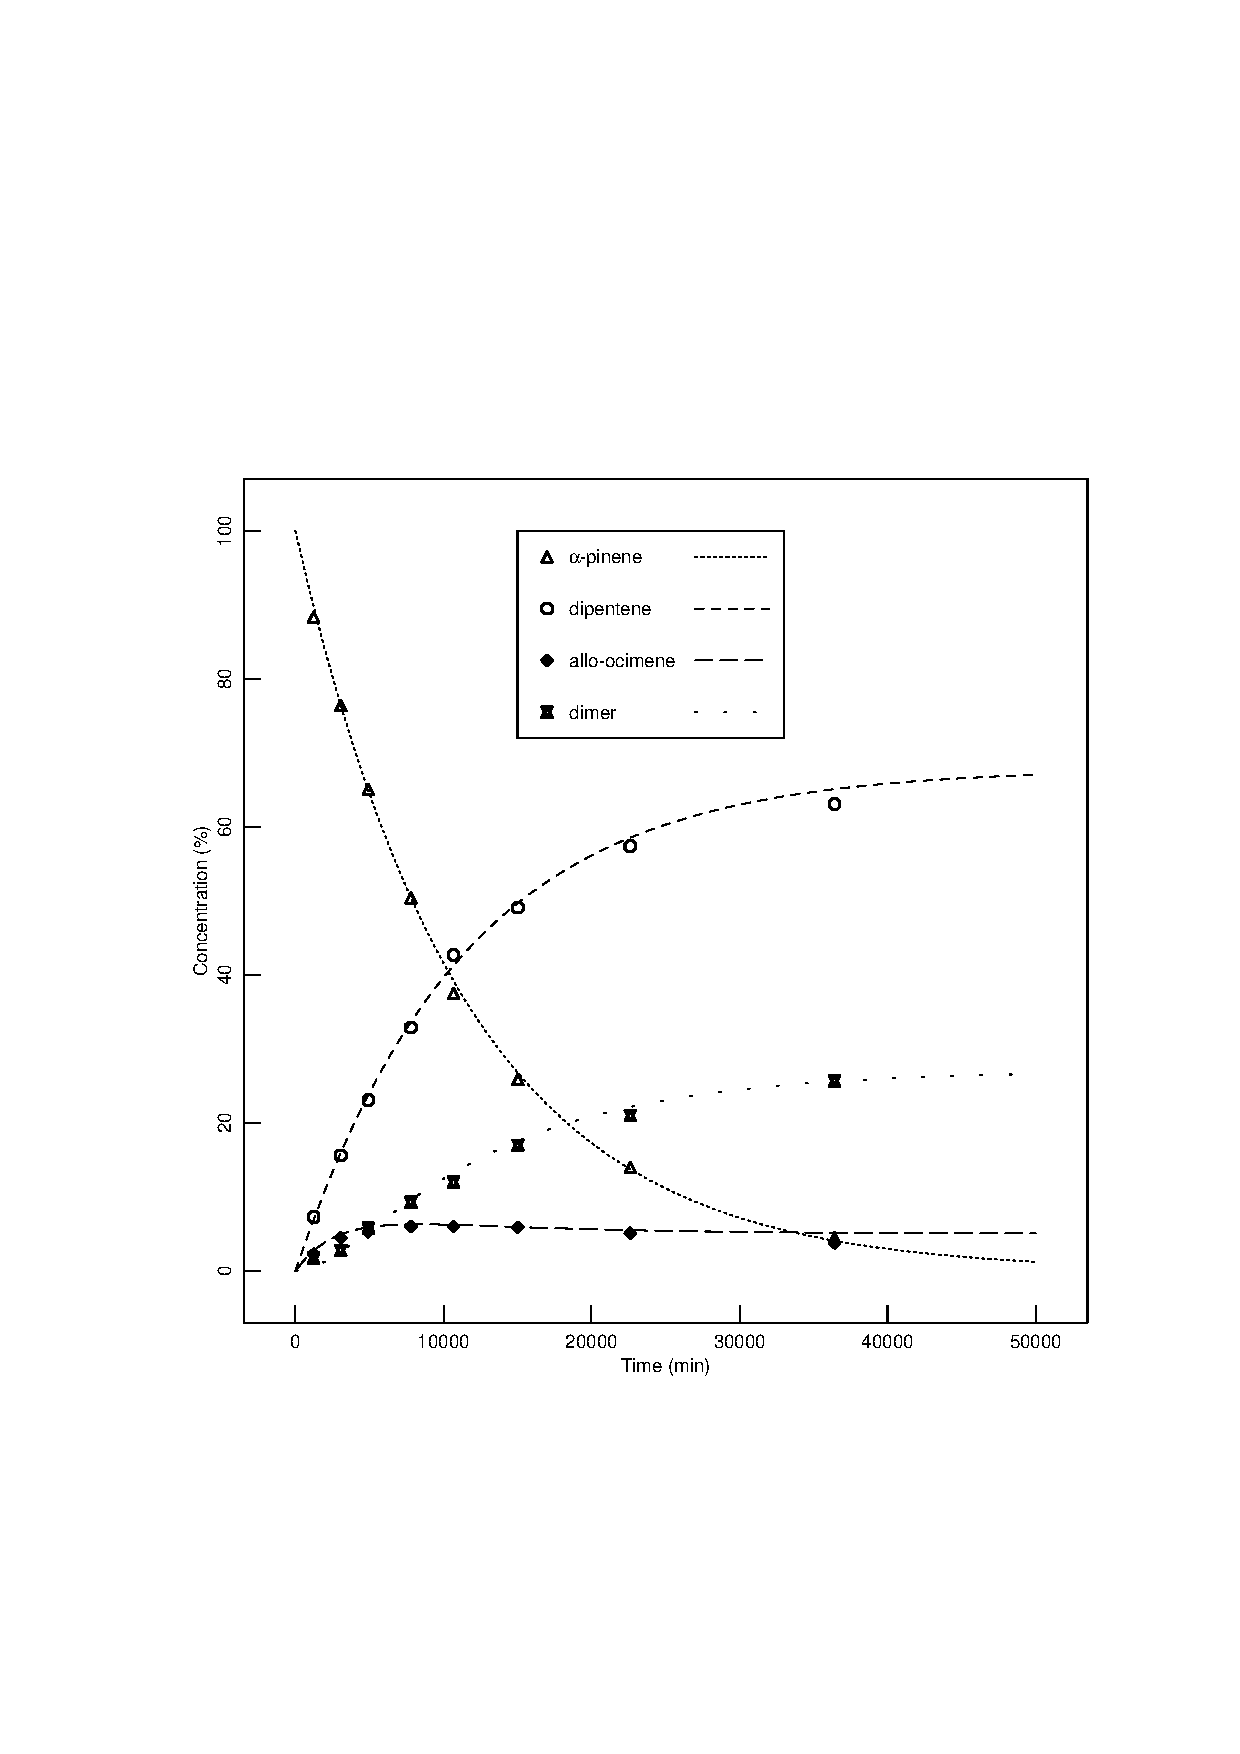
\includegraphics{4BHME4path}}%,height=4.5in}}
  \caption{\label{fig:BHME4path}
  Observed values and the predicted curves obtained by fitting three
  rotated responses to the $\alpha$-pinene data, eliminating pyronene
  production.}
\end{figure}
The residuals for this model are almost identical to those from the
previous fit, and so we could reanalyze the data, treating the
observations with the large residuals as missing.
\end{example}

\begin{problems}
  
  \prob
  Write a computer routine in a language of your choice to
  calculate the determinant, the gradient of the determinant, and the
  approximate Hessian of the determinant, for a multiresponse
  estimation routine.  If necessary, use the pseudocode in Appendix 3,
  Section A3.3 for guidance.
  
  \prob Use the data for responses 1 and 2 in the $\alpha$-pinene data
  set, Appendix 4, Section A4.6, to fit the multiresponse model
  $$
  \bgamma( t )=\left[ \matrix{
      \matrix {e^{{-} ( \theta_1 +\theta_2 )t} \cr
        {\theta_1 \over \theta_1 +\theta_2}
        \left( 1-e^{{-} ( \theta_1 +\theta_2 )t}\right)}
    }\right]
  $$
  Assume the initial concentration of $\alpha$-pinene (response 1)
  is 100\% and of dipentene (response 2) is 0\%.
  
  \subprob Use the approximate rate procedure of Section 4.3.1 to
  obtain starting estimates for the parameters.
  
  \subprob Use a nonlinear estimation routine to obtain the parameter
  estimates.  Replace the missing value for response 1 at time $16020$
  by 0 to obtain the parameter estimates.
  
  \subprob Use the procedure in Section 4.4 to estimate the parameters
  and the missing value.
  
  \prob Perform a singular value decomposition of the centered data
  matrix for the data from Appendix 4, Section A4.7, to determine if
  there are any linear dependencies in the data.
  
  \prob For the data and model of Problem 4.2, the parameter estimates
  and summary statistics from part (b) are as follows:

  \begin{center}
    \begin{tabular}{ccrccc} \hline
      && \multicolumn{3}{c}{Logarithm Scale}\\
      &&& \multicolumn{1}{c}{Std.} & \multicolumn{1}{c}{Correlation}\\
      \multicolumn{1}{c}{Parameter} & \multicolumn{1}{c}{Estimate} &
      \multicolumn{1}{c}{$ln\theta$}& \multicolumn{1}{c}{Error} &
      \multicolumn{1}{c}{Matrix}\\ \hline
      $\theta_{1}$&0.000221&--8.417&0.0085&1.00\\
      $\theta_{2}$&0.000139&--8.881&0.0059&0.69&1.00\\ \hline
    \end{tabular}
  \end{center}

  \subprob Calculate joint and marginal 95\% inference regions for the
  parameters using equations (4.9) and (4.12).
  
  \subprob Use a grid of values of $ln\theta_1 $ from $-8.46$ to
  $-8.38$ in steps 0.005 and $ln\theta_2 $ from $-8.904$ to $-8.854$
  in steps of 0.002, and calculate the determinant at each point.
  Join points of equal value to delineate contours.
  
  \subprob Plot the joint 95\% inference region from part (a) on the
  contour plot in part (b).  Is the linear approximation region
  accurate in this case?
  
  \prob Use the data and model from Appendix 4, Section A4.7 to fit a
  multiresponse model.  Reduce the model to a simple form by
  eliminating parameters which could be zero.  Your analysis to
  Problem 4.3 should have alerted you to the fact that there was a
  dependency in the data.  In fact, the water component $y_{6}$ was
  imputed from a mass balance equation, and so this response should
  not be used in fitting the model.  Because of this, it is convenient
  to estimate the parameters $\theta_{6}$ and $\beta_{6}$ from the
  parameter constraint equations.
\end{problems}


% Local Variables: 
% mode: latex
% TeX-master: "nraia2"
% End: 
